\documentclass[10pt,ignorenonframetext,]{beamer}
\setbeamertemplate{caption}[numbered]
\setbeamertemplate{caption label separator}{: }
\setbeamercolor{caption name}{fg=normal text.fg}

\beamertemplatenavigationsymbolsempty
\usepackage{lmodern}
\usepackage{amssymb,amsmath}
\usepackage{ifxetex,ifluatex}
\usepackage{fixltx2e} % provides \textsubscript
\ifnum 0\ifxetex 1\fi\ifluatex 1\fi=0 % if pdftex
  \usepackage[T1]{fontenc}
  \usepackage[utf8]{inputenc}
\else % if luatex or xelatex
  \ifxetex
    \usepackage{mathspec}
  \else
    \usepackage{fontspec}
  \fi
  \defaultfontfeatures{Ligatures=TeX,Scale=MatchLowercase}
\fi
\usetheme[]{metropolis}
% use upquote if available, for straight quotes in verbatim environments
\IfFileExists{upquote.sty}{\usepackage{upquote}}{}
% use microtype if available
\IfFileExists{microtype.sty}{%
\usepackage{microtype}
\UseMicrotypeSet[protrusion]{basicmath} % disable protrusion for tt fonts
}{}
\newif\ifbibliography
\hypersetup{
            pdftitle={Geospatial Analysis with R},
            pdfauthor={Michael Harper, Luke Blunden},
            pdfborder={0 0 0},
            breaklinks=true}
\urlstyle{same}  % don't use monospace font for urls
\usepackage{color}
\usepackage{fancyvrb}
\newcommand{\VerbBar}{|}
\newcommand{\VERB}{\Verb[commandchars=\\\{\}]}
\DefineVerbatimEnvironment{Highlighting}{Verbatim}{commandchars=\\\{\}}
% Add ',fontsize=\small' for more characters per line
\usepackage{framed}
\definecolor{shadecolor}{RGB}{248,248,248}
\newenvironment{Shaded}{\begin{snugshade}}{\end{snugshade}}
\newcommand{\KeywordTok}[1]{\textcolor[rgb]{0.13,0.29,0.53}{\textbf{{#1}}}}
\newcommand{\DataTypeTok}[1]{\textcolor[rgb]{0.13,0.29,0.53}{{#1}}}
\newcommand{\DecValTok}[1]{\textcolor[rgb]{0.00,0.00,0.81}{{#1}}}
\newcommand{\BaseNTok}[1]{\textcolor[rgb]{0.00,0.00,0.81}{{#1}}}
\newcommand{\FloatTok}[1]{\textcolor[rgb]{0.00,0.00,0.81}{{#1}}}
\newcommand{\ConstantTok}[1]{\textcolor[rgb]{0.00,0.00,0.00}{{#1}}}
\newcommand{\CharTok}[1]{\textcolor[rgb]{0.31,0.60,0.02}{{#1}}}
\newcommand{\SpecialCharTok}[1]{\textcolor[rgb]{0.00,0.00,0.00}{{#1}}}
\newcommand{\StringTok}[1]{\textcolor[rgb]{0.31,0.60,0.02}{{#1}}}
\newcommand{\VerbatimStringTok}[1]{\textcolor[rgb]{0.31,0.60,0.02}{{#1}}}
\newcommand{\SpecialStringTok}[1]{\textcolor[rgb]{0.31,0.60,0.02}{{#1}}}
\newcommand{\ImportTok}[1]{{#1}}
\newcommand{\CommentTok}[1]{\textcolor[rgb]{0.56,0.35,0.01}{\textit{{#1}}}}
\newcommand{\DocumentationTok}[1]{\textcolor[rgb]{0.56,0.35,0.01}{\textbf{\textit{{#1}}}}}
\newcommand{\AnnotationTok}[1]{\textcolor[rgb]{0.56,0.35,0.01}{\textbf{\textit{{#1}}}}}
\newcommand{\CommentVarTok}[1]{\textcolor[rgb]{0.56,0.35,0.01}{\textbf{\textit{{#1}}}}}
\newcommand{\OtherTok}[1]{\textcolor[rgb]{0.56,0.35,0.01}{{#1}}}
\newcommand{\FunctionTok}[1]{\textcolor[rgb]{0.00,0.00,0.00}{{#1}}}
\newcommand{\VariableTok}[1]{\textcolor[rgb]{0.00,0.00,0.00}{{#1}}}
\newcommand{\ControlFlowTok}[1]{\textcolor[rgb]{0.13,0.29,0.53}{\textbf{{#1}}}}
\newcommand{\OperatorTok}[1]{\textcolor[rgb]{0.81,0.36,0.00}{\textbf{{#1}}}}
\newcommand{\BuiltInTok}[1]{{#1}}
\newcommand{\ExtensionTok}[1]{{#1}}
\newcommand{\PreprocessorTok}[1]{\textcolor[rgb]{0.56,0.35,0.01}{\textit{{#1}}}}
\newcommand{\AttributeTok}[1]{\textcolor[rgb]{0.77,0.63,0.00}{{#1}}}
\newcommand{\RegionMarkerTok}[1]{{#1}}
\newcommand{\InformationTok}[1]{\textcolor[rgb]{0.56,0.35,0.01}{\textbf{\textit{{#1}}}}}
\newcommand{\WarningTok}[1]{\textcolor[rgb]{0.56,0.35,0.01}{\textbf{\textit{{#1}}}}}
\newcommand{\AlertTok}[1]{\textcolor[rgb]{0.94,0.16,0.16}{{#1}}}
\newcommand{\ErrorTok}[1]{\textcolor[rgb]{0.64,0.00,0.00}{\textbf{{#1}}}}
\newcommand{\NormalTok}[1]{{#1}}

% Prevent slide breaks in the middle of a paragraph:
\widowpenalties 1 10000
\raggedbottom

\AtBeginPart{
  \let\insertpartnumber\relax
  \let\partname\relax
  \frame{\partpage}
}
\AtBeginSection{
  \ifbibliography
  \else
    \let\insertsectionnumber\relax
    \let\sectionname\relax
    \frame{\sectionpage}
  \fi
}
\AtBeginSubsection{
  \let\insertsubsectionnumber\relax
  \let\subsectionname\relax
  \frame{\subsectionpage}
}

\setlength{\parindent}{0pt}
\setlength{\parskip}{6pt plus 2pt minus 1pt}
\setlength{\emergencystretch}{3em}  % prevent overfull lines
\providecommand{\tightlist}{%
  \setlength{\itemsep}{0pt}\setlength{\parskip}{0pt}}
\setcounter{secnumdepth}{0}
\def\begincols{\begin{columns}}
\def\begincol{\begin{column}}
\def\endcol{\end{column}}
\def\endcols{\end{columns}}

% Style Blocks
\definecolor{BlueTOL}{HTML}{222255}
\definecolor{BrownTOL}{HTML}{666633}
\definecolor{GreenTOL}{HTML}{225522}
\definecolor{shadecolor}{RGB}{255,255,255}
\setbeamercolor{alerted text}{fg=BrownTOL}
\setbeamercolor{example text}{fg=GreenTOL}

\setbeamercolor{block title alerted}{use=alerted text,
    fg=alerted text.fg,
    bg=alerted text.bg!80!alerted text.fg}
\setbeamercolor{block body alerted}{use={block title alerted, alerted text},
    fg=alerted text.fg,
    bg=block title alerted.bg!50!alerted text.bg}
\setbeamercolor{block title example}{use=example text,
    fg=example text.fg,
    bg=example text.bg!80!example text.fg}
\setbeamercolor{block body example}{use={block title example, example text},
    fg=example text.fg,
    bg=block title example.bg!50!example text.bg}
    
% Custom Content
\setbeamertemplate{frame footer}{Geospatial Data with R}
\setbeamertemplate{navigation symbols}{}
\setbeamertemplate{footline}[page number]

\setbeamercolor{block title}{use=structure,fg=black,bg=BlueTOL}
\setbeamercolor{block body}{use=structure,fg=white,bg=white!20!white}

% change the font size of verbatim text
\makeatletter
\def\verbatim{\small\@verbatim \frenchspacing\@vobeyspaces \@xverbatim}
\makeatother

\title{Geospatial Analysis with R}
\author{Michael Harper, Luke Blunden}
\institute{University of Southampton}
\date{\today}

\begin{document}
\frame{\titlepage}

\begin{frame}{Uses of Spatial Data in Science}

\begincols
\begincol{.48\textwidth}

\begin{itemize}
\tightlist
\item
  spatial analysis: using location or spatial relationships as an
  \textbf{explanatory} or \textbf{predictive} variable
\item
  examining the effects of \textbf{scale}
\item
  backdrops to show \textbf{context}
\end{itemize}

\endcol
\begincol{.48\textwidth}

\begin{figure}

{\centering 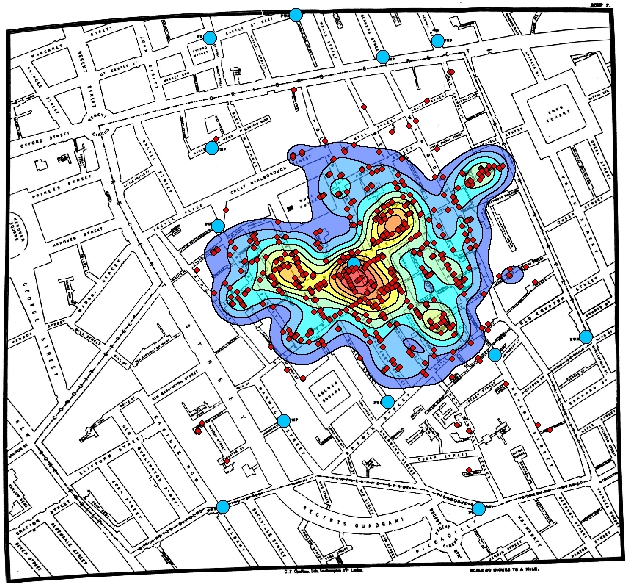
\includegraphics[width=1\linewidth]{../images/cholera_kernel_density} 

}

\caption{Cholera Map of 1854 London Outbreak}\label{fig:unnamed-chunk-1}
\end{figure}

\endcol
\endcols

\end{frame}

\begin{frame}{GIS vs.~R}

\begin{itemize}
\tightlist
\item
  Many tools options also available
\end{itemize}

\begincols
\begincol{.48\textwidth}

\begin{center}
\includegraphics[width=0.8\linewidth]{../images/arcgis} \end{center}

\endcol
\begincol{.48\textwidth}

\begin{center}
\includegraphics[width=0.5\linewidth]{../images/RLogo} \end{center}

\endcol
\endcols

\begin{itemize}
\tightlist
\item
  Other tools avaialble (QGIS, Python)
\end{itemize}

\begin{alertblock}{Which tool is best to use?}
Well, it depends on the task!
\end{alertblock}

\end{frame}

\begin{frame}{GIS vs.~R}

\begincols
\begincol{.48\textwidth}

\textbf{GIS}

\begin{itemize}
\tightlist
\item
  Visual interaction
\item
  Data management
\item
  Geometric operations
\item
  Standard workflows
\item
  Single map production
\item
  Click, click, click, click
\item
  Speed of execution
\end{itemize}

\endcol
\begincol{.48\textwidth}

\textbf{R}

\begin{itemize}
\tightlist
\item
  Data and model focused
\item
  Analysis
\item
  Attributes as important
\item
  Creativity and innovation
\item
  Many (simpler) maps
\item
  Repeatability (script)
\item
  Speed of development
\end{itemize}

\endcol
\endcols

\end{frame}

\begin{frame}{R Examples (1)}

\begin{figure}

{\centering 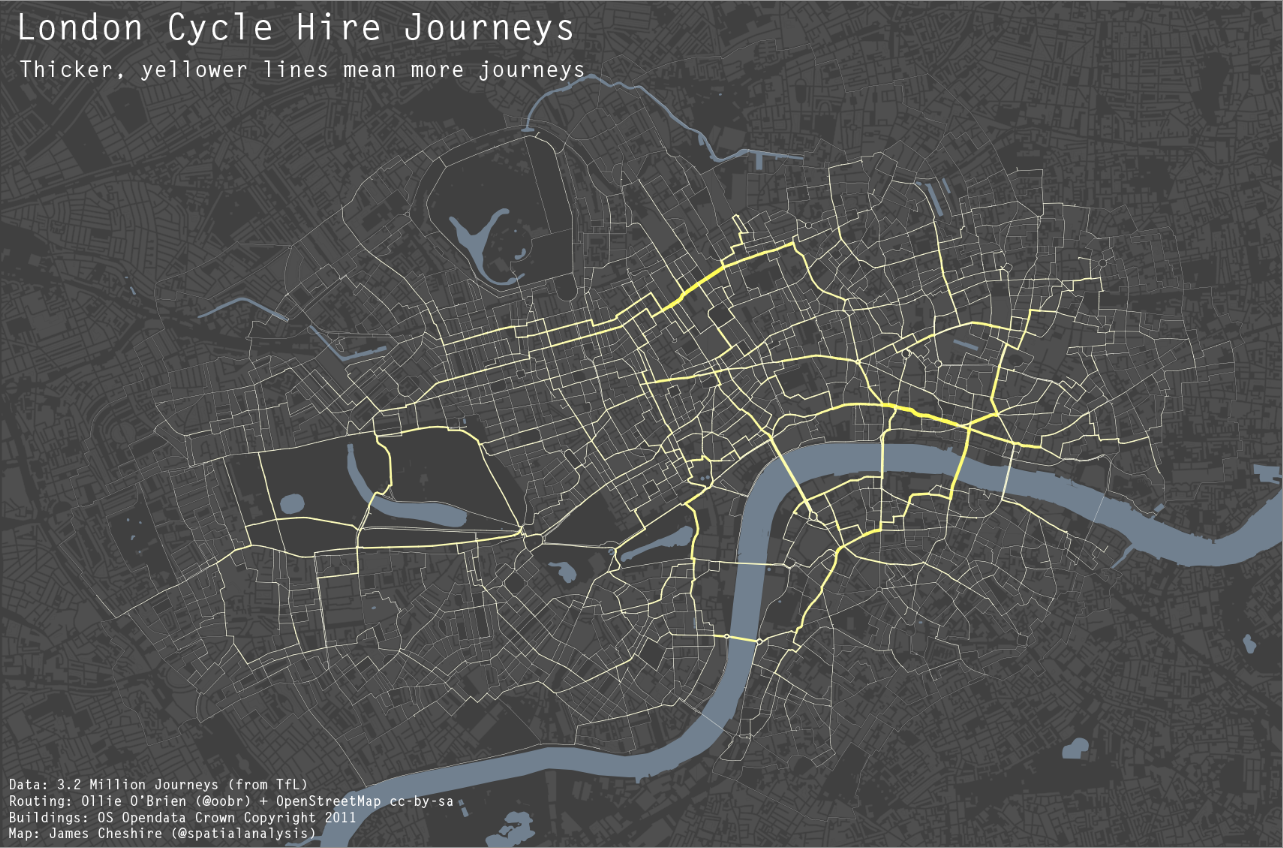
\includegraphics[width=0.9\linewidth]{../images/bike_ggplot} 

}

\caption{London Cycle Hire Journeys}\label{fig:unnamed-chunk-4}
\end{figure}

\url{http://spatial.ly/2012/02/great-maps-ggplot2/}

\end{frame}

\begin{frame}{R Examples (2)}

\begin{figure}

{\centering 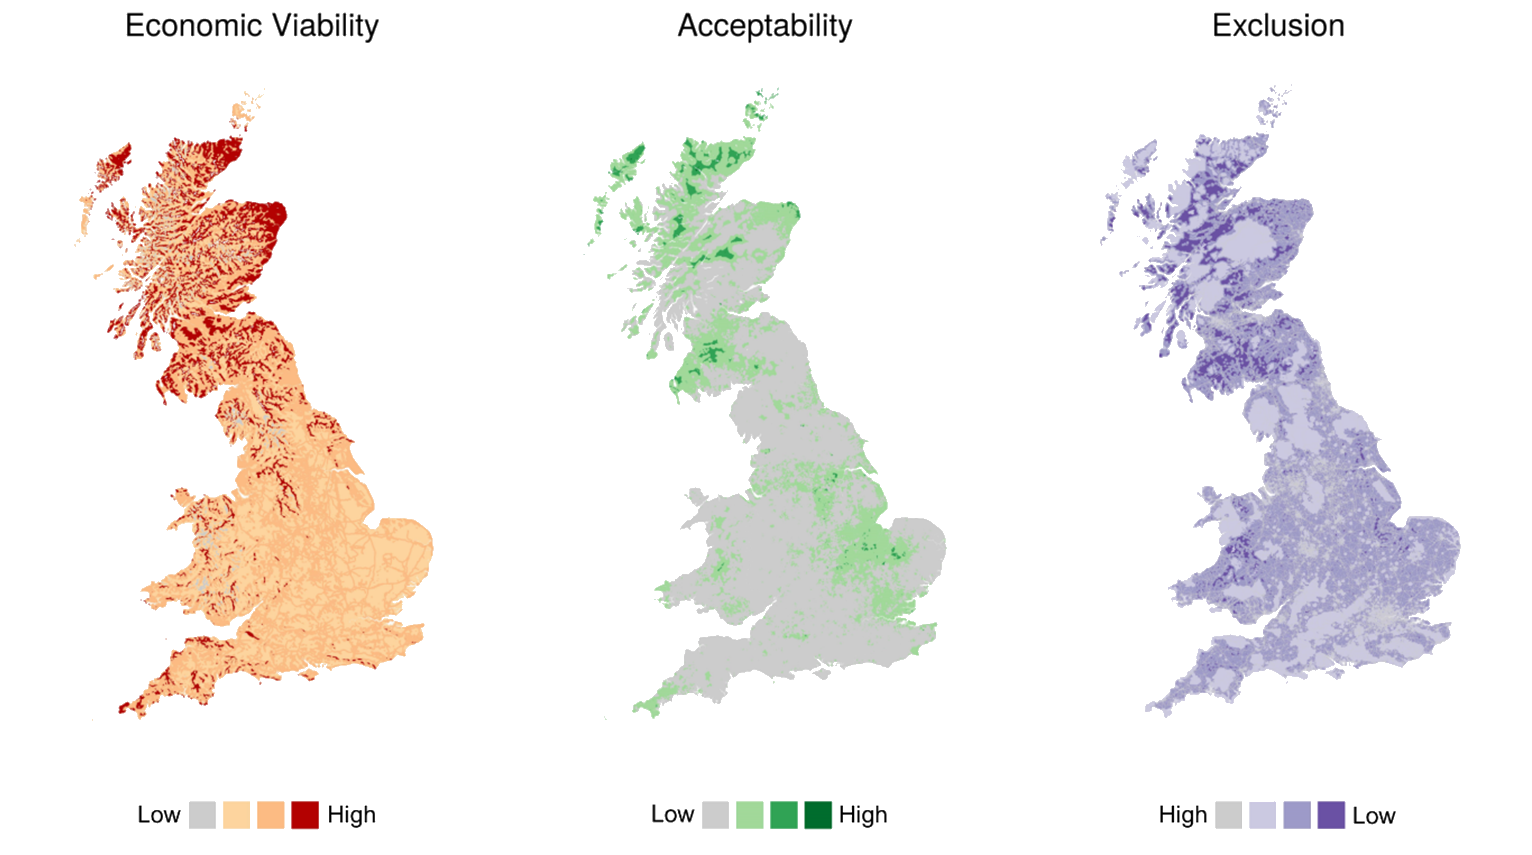
\includegraphics[width=1\linewidth]{../images/WindTurbineStudies} 

}

\caption{Wind Turbine Analysis of Great Britain}\label{fig:unnamed-chunk-5}
\end{figure}

\end{frame}

\begin{frame}{Challenges with Spatial Data in R}

\textbf{Understanding and manipulating spatial data in R can be a real
challenge!}

\begincols
\begincol{.48\textwidth}

\begin{itemize}
\tightlist
\item
  Many types and formats of spatial data
\item
  R is not the easiest program to learn
\item
  There are a many packages from a very diverse user community
\end{itemize}

\endcol
\begincol{.48\textwidth}

\begin{center}
\includegraphics[width=0.8\linewidth]{../images/alert_icon} \end{center}

\endcol
\endcols

\end{frame}

\begin{frame}{Presentation Goals}

\begincols
\begincol{.69\textwidth}

\begin{enumerate}
\def\labelenumi{\arabic{enumi}.}
\tightlist
\item
  Help you get to the point where you can do basic analysis or
  visualization
\item
  Point out some of the commonly-used packages for spatial data
  manipulation and analysis
\item
  Be a resource you can come back to
\item
  Provide Guidance on useful resources to use after the course
\end{enumerate}

\endcol
\begincol{.3\textwidth}

\begin{center}
\includegraphics[width=1\linewidth]{../images/Goals} \end{center}

\endcol
\endcols

\begin{alertblock}{Beware of the learning curve!}
Takes patience to master.
\end{alertblock}

\end{frame}

\begin{frame}{Outline}

\begincols
\begincol{.7\textwidth}

\begin{enumerate}
\def\labelenumi{\arabic{enumi}.}
\tightlist
\item
  Creating Spatial Objects
\item
  Data Table Operations
\item
  Coordinate Systems and Reprojection
\item
  Geoprocessing
\item
  Presenting Results
\end{enumerate}

\endcol
\begincol{.3\textwidth}

\endcol
\endcols

\begin{alertblock}{Subjects Omitted}
More advanced visualization, Spatial statistics, Geodatabases, Network analysis, Many other...
\end{alertblock}

\end{frame}

\begin{frame}[fragile]{Before We Start\ldots{}}

\begin{itemize}
\tightlist
\item
  Many packages are used within the analysis.
\end{itemize}

\begin{Shaded}
\begin{Highlighting}[]
\KeywordTok{library}\NormalTok{(rgdal)  }\CommentTok{# loads geospatial libraries}
\KeywordTok{library}\NormalTok{(rgeos)  }\CommentTok{# dealing with geospatial files}
\KeywordTok{library}\NormalTok{(sp)  }\CommentTok{# spatial projections}
\KeywordTok{library}\NormalTok{(raster)  }\CommentTok{# loading rasters and geoprocessing}
\KeywordTok{library}\NormalTok{(ggplot2)  }\CommentTok{# Creating maps}
\KeywordTok{library}\NormalTok{(spatstat)  }\CommentTok{# Used for spatial statistics}
\end{Highlighting}
\end{Shaded}

\begin{itemize}
\tightlist
\item
  Don't worry for now. These will be explained in more detail later.
\end{itemize}

\end{frame}

\section{PART I: Creating Spatial
Objects}\label{part-i-creating-spatial-objects}

\begin{frame}{Representing Physical Features}

\begincols
\begincol{.4\textwidth}

\begin{figure}

{\centering 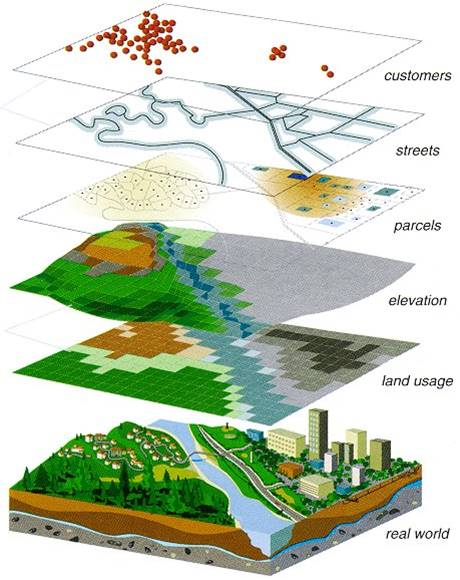
\includegraphics[width=1\linewidth]{../images/layers} 

}

\caption{Representation of Figure Layers}\label{fig:unnamed-chunk-9}
\end{figure}

\endcol
\begincol{.49\textwidth}

\begin{figure}

{\centering 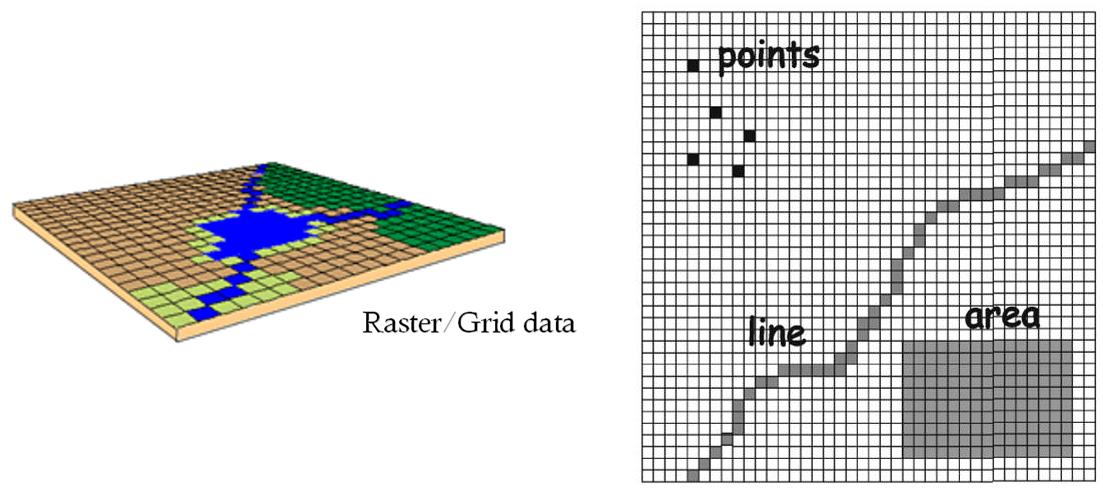
\includegraphics[width=1\linewidth]{../images/raster-features-abstract} 

}

\caption{Raster Features}\label{fig:unnamed-chunk-10}
\end{figure}

\begin{figure}

{\centering 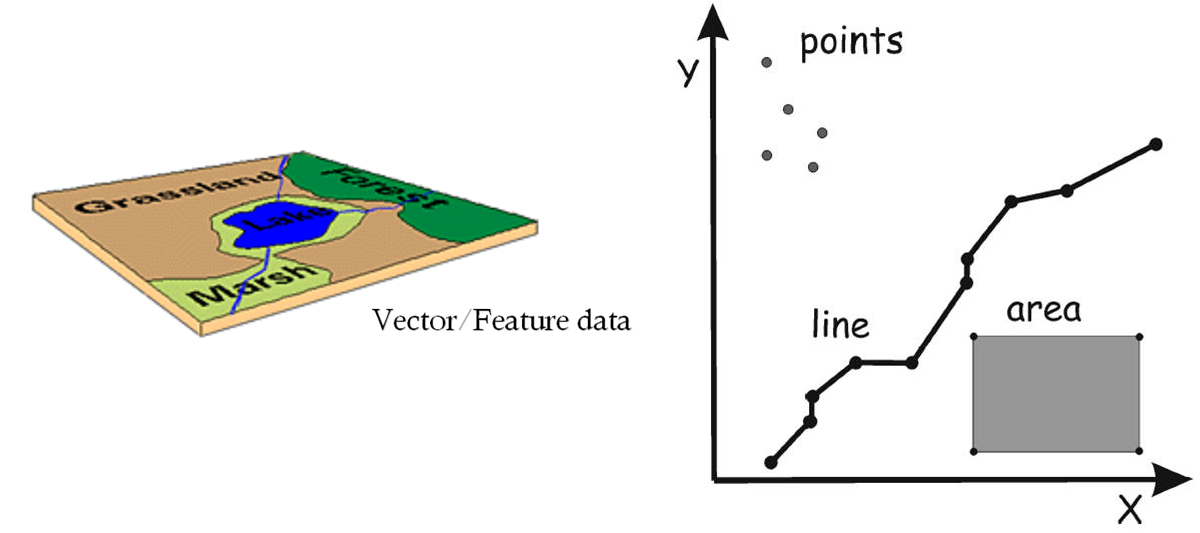
\includegraphics[width=1\linewidth]{../images/vectors-features-abstract} 

}

\caption{Vector Features}\label{fig:unnamed-chunk-11}
\end{figure}

\endcol
\endcols

\end{frame}

\begin{frame}[fragile]{Creating SpatialPoints Objects}

\begin{itemize}
\tightlist
\item
  The package \alert{sp} is primarily used for creating spatial data
  types
\item
  The code
  \texttt{getClass(\textquotesingle{}Spatial\textquotesingle{})} can be
  run to see all types
\end{itemize}

Three options to create spatial data in R:

\begin{enumerate}
\def\labelenumi{\arabic{enumi}.}
\tightlist
\item
  Create from scratch
\item
  Promote a data frame with X and Y columns
\item
  Import a GIS file
\end{enumerate}

\begin{itemize}
\tightlist
\item
  Methods 2 and 3 are most commonly used!
\item
  Tutorial will focus on creation of Points
\end{itemize}

\end{frame}

\begin{frame}[fragile]{Method 1: Create a SpatialPoints Object from
Scratch}

\begin{itemize}
\tightlist
\item
  Let's create an example dataset!
\end{itemize}

\begin{Shaded}
\begin{Highlighting}[]
\KeywordTok{library}\NormalTok{(sp)}
\CommentTok{# create a set of random coordinates}
\NormalTok{xy <-}\StringTok{ }\KeywordTok{matrix}\NormalTok{(}\DataTypeTok{data =} \KeywordTok{runif}\NormalTok{(}\DataTypeTok{n =} \DecValTok{100}\NormalTok{), }\DataTypeTok{ncol =} \DecValTok{2}\NormalTok{)}
\KeywordTok{head}\NormalTok{(xy, }\DataTypeTok{n =} \DecValTok{3}\NormalTok{)  }\CommentTok{# show first three rows}
\end{Highlighting}
\end{Shaded}

\begin{verbatim}
##            [,1]      [,2]
## [1,] 0.03463934 0.6675732
## [2,] 0.15650207 0.1940877
## [3,] 0.44065106 0.1272320
\end{verbatim}

\begin{itemize}
\tightlist
\item
  \texttt{SpatialPoints} function can be used to create a dataset from
  XY coordinates
\end{itemize}

\begin{Shaded}
\begin{Highlighting}[]
\NormalTok{xySp <-}\StringTok{ }\KeywordTok{SpatialPoints}\NormalTok{(xy)}
\end{Highlighting}
\end{Shaded}

\end{frame}

\begin{frame}[fragile]{Method 1: Create a SpatialPoints Object from
Scratch}

SpatialPoints can be plotted as typical XY data using the
\texttt{plot()} function

\begin{Shaded}
\begin{Highlighting}[]
\KeywordTok{plot}\NormalTok{(xySp, }\DataTypeTok{axes =} \OtherTok{TRUE}\NormalTok{, }\DataTypeTok{main =} \StringTok{"Example Spatial Data Points"}\NormalTok{)}
\end{Highlighting}
\end{Shaded}

\begin{center}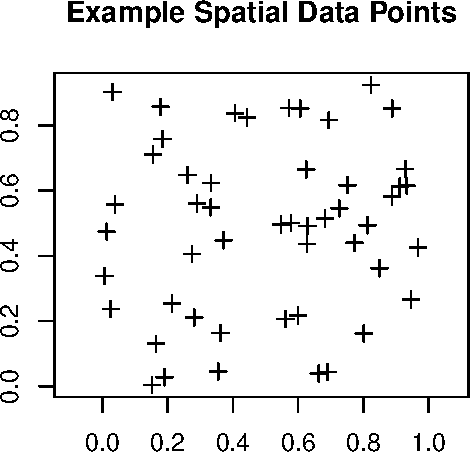
\includegraphics[width=0.5\linewidth]{SpatialDataLecture_files/figure-beamer/plotxy-1} \end{center}

\end{frame}

\begin{frame}[fragile]{Method 2: Promote a DataFrame to a
SpatialPointsDataFrame}

\begin{itemize}
\tightlist
\item
  It is unlikely you will use Method 1 often
\item
  You will more likely have an existing dataset with XY coordinates.
\item
  For the tutorial, We will used the \alert{canada.cities} dataset from
  the \alert{maps} package.
\end{itemize}

\begin{Shaded}
\begin{Highlighting}[]
\KeywordTok{library}\NormalTok{(maps)}
\KeywordTok{head}\NormalTok{(canada.cities, }\DataTypeTok{n =} \DecValTok{3}\NormalTok{)}
\end{Highlighting}
\end{Shaded}

\begin{verbatim}
##            name country.etc    pop   lat    long capital
## 1 Abbotsford BC          BC 157795 49.06 -122.30       0
## 2      Acton ON          ON   8308 43.63  -80.03       0
## 3 Acton Vale QC          QC   5153 45.63  -72.57       0
\end{verbatim}

\begin{itemize}
\tightlist
\item
  Data already has X (long) and Y (lat) references.
\end{itemize}

\end{frame}

\begin{frame}[fragile]{Method 2: Promote a DataFrame to a
SpatialPointsDataFrame}

\begin{itemize}
\tightlist
\item
  We must let R know which columns are the X and Y coordinates
\end{itemize}

\begin{Shaded}
\begin{Highlighting}[]
\CommentTok{# Create a new variable to edit the data}
\NormalTok{cities <-}\StringTok{ }\NormalTok{canada.cities}

\CommentTok{# State which columns contain the x and y}
\CommentTok{# coordinates}
\KeywordTok{coordinates}\NormalTok{(cities) <-}\StringTok{ }\ErrorTok{~}\NormalTok{long +}\StringTok{ }\NormalTok{lat}
\end{Highlighting}
\end{Shaded}

\begin{itemize}
\tightlist
\item
  By assigning coordinates we create a SpatialPointsDataFrame:
\end{itemize}

\begin{Shaded}
\begin{Highlighting}[]
\KeywordTok{class}\NormalTok{(cities)}
\end{Highlighting}
\end{Shaded}

\begin{verbatim}
## [1] "SpatialPointsDataFrame"
## attr(,"package")
## [1] "sp"
\end{verbatim}

\end{frame}

\begin{frame}[fragile]{Method 2: Promote a DataFrame to a
SpatialPointsDataFrame}

We can map the results of the SpatialDataFrame as before:

\begin{Shaded}
\begin{Highlighting}[]
\KeywordTok{plot}\NormalTok{(cities, }\DataTypeTok{axes =} \OtherTok{TRUE}\NormalTok{, }\DataTypeTok{main =} \StringTok{"Cities in Canada"}\NormalTok{, }
    \DataTypeTok{xlab =} \StringTok{"Longitude"}\NormalTok{, }\DataTypeTok{ylab =} \StringTok{"Latitude"}\NormalTok{)}
\end{Highlighting}
\end{Shaded}

\begin{center}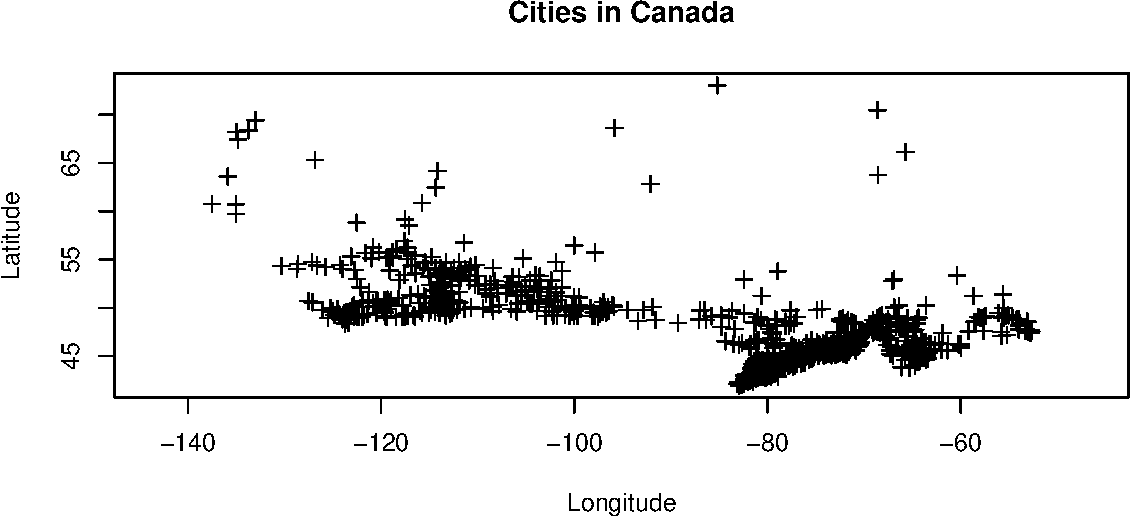
\includegraphics[width=0.8\linewidth]{SpatialDataLecture_files/figure-beamer/unnamed-chunk-13-1} \end{center}

\begin{itemize}
\tightlist
\item
  This map is not very useful yet! We will add to this map later!
\end{itemize}

\end{frame}

\begin{frame}[fragile]{Method 3: Import a GIS File}

\begin{itemize}
\tightlist
\item
  Package \alert{rgdal} has a large set of import and export filters for
  both vector and raster GIS data (Shapefiles, KML, GPX etc.).
\item
  For the complete list of vector import filters, use the function
  \texttt{ogrDrivers()}.
\item
  The tutorial will focus on \textbf{Shapefiles}, a commonly used format
  in GIS software.
\item
  We will use the ``scot\_BNG'' file.
\item
  \texttt{readOGR()} is the function you use to import a vector file.
\end{itemize}

\begin{Shaded}
\begin{Highlighting}[]
\CommentTok{# Find the file path of the vectors}
\NormalTok{vectorDir <-}\StringTok{ }\KeywordTok{system.file}\NormalTok{(}\StringTok{"vectors"}\NormalTok{, }\DataTypeTok{package =} \StringTok{"rgdal"}\NormalTok{)}
\NormalTok{scotland <-}\StringTok{ }\KeywordTok{readOGR}\NormalTok{(}\DataTypeTok{dsn =} \NormalTok{vectorDir, }\DataTypeTok{layer =} \StringTok{"scot_BNG"}\NormalTok{, }
    \DataTypeTok{verbose =} \OtherTok{FALSE}\NormalTok{)}
\end{Highlighting}
\end{Shaded}

\begin{itemize}
\tightlist
\item
  Note: you don't need to include the file extension when loading the
  object
\end{itemize}

\end{frame}

\begin{frame}[fragile]{Method 3: Import a GIS File}

\begin{itemize}
\tightlist
\item
  Shapefiles are typically easy to plot straight away
\end{itemize}

\begin{Shaded}
\begin{Highlighting}[]
\KeywordTok{plot}\NormalTok{(scotland, }\DataTypeTok{axes =} \NormalTok{T, }\DataTypeTok{asp =} \DecValTok{1}\NormalTok{, }\DataTypeTok{col =} \KeywordTok{palette}\NormalTok{())}
\end{Highlighting}
\end{Shaded}

\begin{center}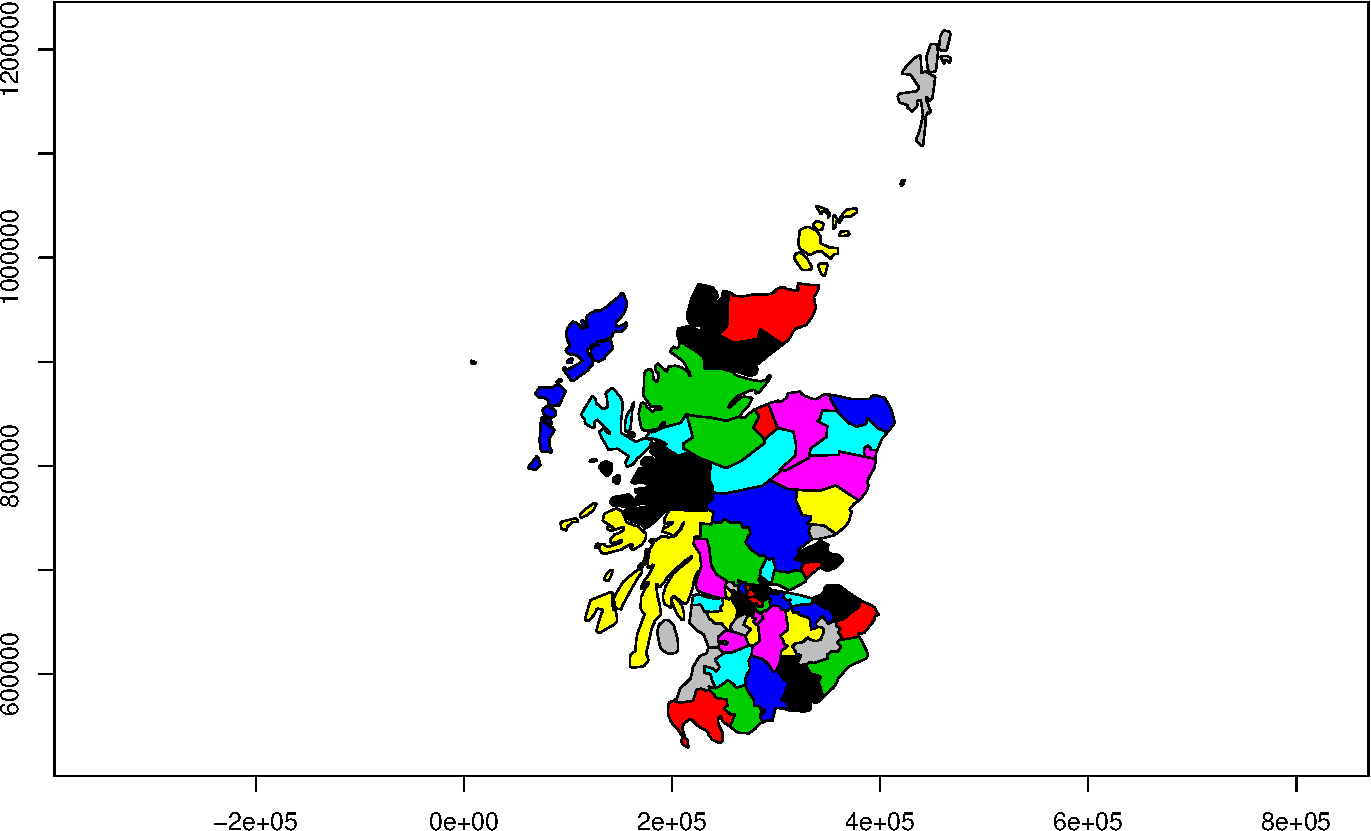
\includegraphics[width=0.8\linewidth]{SpatialDataLecture_files/figure-beamer/plot_scotland-1} \end{center}

\begin{itemize}
\tightlist
\item
  We will come back to plotting again later!
\end{itemize}

\end{frame}

\section{PART II: Working With
SpatialDataFrames}\label{part-ii-working-with-spatialdataframes}

\begin{frame}[fragile]{Working with the Data Frame}

\begin{itemize}
\tightlist
\item
  You can work with the data frame as you would with any data frame
\item
  To use the attribute table of a SpatialPointsDataFrame, use the
  \textbf{data} slot (with `@' character):
\end{itemize}

\begincols
\begincol{.48\textwidth}

\begin{Shaded}
\begin{Highlighting}[]
\KeywordTok{nrow}\NormalTok{(cities@data)}
\end{Highlighting}
\end{Shaded}

\begin{verbatim}
## [1] 916
\end{verbatim}

\endcol
\begincol{.48\textwidth}

\begin{Shaded}
\begin{Highlighting}[]
\CommentTok{# show the column names}
\KeywordTok{names}\NormalTok{(cities@data)}
\end{Highlighting}
\end{Shaded}

\begin{verbatim}
## [1] "name"        "country.etc" "pop"         "capital"
\end{verbatim}

\endcol
\endcols

\begin{itemize}
\tightlist
\item
  What happened to the coordinates?
\item
  We can read them with the \texttt{coordinates()} function
\end{itemize}

\begin{Shaded}
\begin{Highlighting}[]
\KeywordTok{coordinates}\NormalTok{(cities)[}\DecValTok{1}\NormalTok{, ]}
\end{Highlighting}
\end{Shaded}

\begin{verbatim}
##    long     lat 
## -122.30   49.06
\end{verbatim}

\end{frame}

\begin{frame}[fragile]{Calculating Summaries}

\begin{itemize}
\tightlist
\item
  SpatialDataframes can \emph{mostly} be treated like a normal Dataframe
\end{itemize}

\begin{Shaded}
\begin{Highlighting}[]
\KeywordTok{mean}\NormalTok{(cities$pop)  }\CommentTok{# Calculate Mean population}
\end{Highlighting}
\end{Shaded}

\begin{verbatim}
## [1] 27463.94
\end{verbatim}

\begin{Shaded}
\begin{Highlighting}[]
\NormalTok{ggplot2::}\KeywordTok{qplot}\NormalTok{(}\DataTypeTok{x =} \StringTok{""}\NormalTok{, }\DataTypeTok{y =} \NormalTok{cities$pop, }\DataTypeTok{geom =} \StringTok{"boxplot"}\NormalTok{, }
    \DataTypeTok{main =} \StringTok{"A questionable boxplot"}\NormalTok{, }\DataTypeTok{ylab =} \StringTok{"Population"}\NormalTok{) +}\StringTok{ }
\StringTok{    }\KeywordTok{coord_flip}\NormalTok{()}
\end{Highlighting}
\end{Shaded}

\begin{center}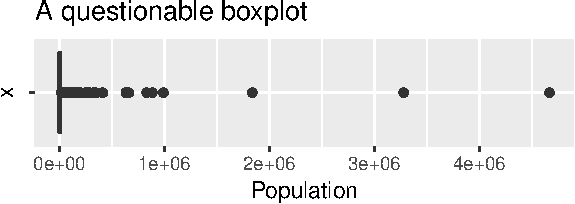
\includegraphics[width=0.8\linewidth]{SpatialDataLecture_files/figure-beamer/unnamed-chunk-17-1} \end{center}

\end{frame}

\begin{frame}[fragile]{Adding a Column to the Data Frame of a SPDF
Object}

\begin{itemize}
\tightlist
\item
  Calculate new columns in the data frame
\end{itemize}

\begin{Shaded}
\begin{Highlighting}[]
\CommentTok{# Calculate the size order of cities}
\NormalTok{cities$sizerank <-}\StringTok{ }\KeywordTok{rank}\NormalTok{(-cities$pop)}

\KeywordTok{head}\NormalTok{(cities@data, }\DataTypeTok{n =} \DecValTok{5}\NormalTok{)}
\end{Highlighting}
\end{Shaded}

\begin{verbatim}
##            name country.etc    pop capital sizerank
## 1 Abbotsford BC          BC 157795       0       20
## 2      Acton ON          ON   8308       0      220
## 3 Acton Vale QC          QC   5153       0      314
## 4    Airdrie AB          AB  25863       0       86
## 5    Aklavik NT          NT    643       0      915
\end{verbatim}

\end{frame}

\begin{frame}[fragile]{Filter on an Attribute}

\begin{itemize}
\tightlist
\item
  Standard R syntax can be used to filter
  SpatialDataFrames.\footnote<.->{Check out
    \url{http://www.statmethods.net/management/subset.html}}
\end{itemize}

\begin{Shaded}
\begin{Highlighting}[]
\CommentTok{# Filter cities by those with a population more}
\CommentTok{# than 100,000}
\NormalTok{BigCities <-}\StringTok{ }\NormalTok{cities[cities$pop >}\StringTok{ }\FloatTok{1e+05}\NormalTok{, ]}

\CommentTok{# Count how many cities meet criteria}
\KeywordTok{nrow}\NormalTok{(BigCities)}
\end{Highlighting}
\end{Shaded}

\begin{verbatim}
## [1] 29
\end{verbatim}

\end{frame}

\begin{frame}[fragile]{Filter on an Attribute}

\small

\begin{Shaded}
\begin{Highlighting}[]
\KeywordTok{par}\NormalTok{(}\DataTypeTok{mfrow =} \KeywordTok{c}\NormalTok{(}\DecValTok{1}\NormalTok{, }\DecValTok{2}\NormalTok{))  }\CommentTok{# Plot graphs side by side}
\KeywordTok{plot}\NormalTok{(cities, }\DataTypeTok{axes =} \NormalTok{T, }\DataTypeTok{asp =} \DecValTok{1}\NormalTok{, }\DataTypeTok{pch =} \DecValTok{16}\NormalTok{, }\DataTypeTok{main =} \StringTok{"Original"}\NormalTok{)}
\KeywordTok{plot}\NormalTok{(cities, }\DataTypeTok{axes =} \NormalTok{T, }\DataTypeTok{asp =} \DecValTok{1}\NormalTok{, }\DataTypeTok{pch =} \DecValTok{16}\NormalTok{, }\DataTypeTok{main =} \StringTok{"Highlighing Big Cities"}\NormalTok{)}
\KeywordTok{plot}\NormalTok{(BigCities, }\DataTypeTok{pch =} \DecValTok{1}\NormalTok{, }\DataTypeTok{col =} \StringTok{"red"}\NormalTok{, }\DataTypeTok{cex =} \DecValTok{3}\NormalTok{, }\DataTypeTok{add =} \OtherTok{TRUE}\NormalTok{)}
\end{Highlighting}
\end{Shaded}

\begin{figure}

{\centering 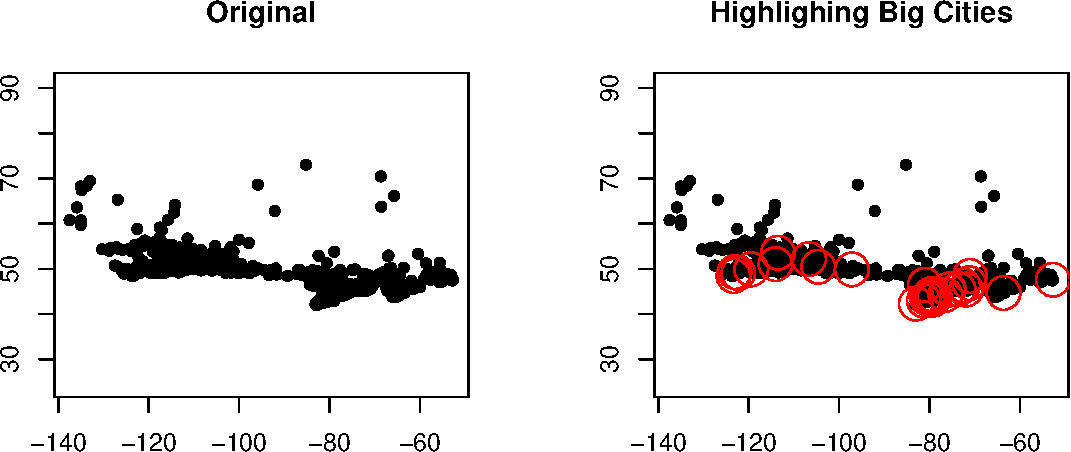
\includegraphics[width=1\linewidth]{SpatialDataLecture_files/figure-beamer/unnamed-chunk-19-1} 

}

\caption{Subsetting of spatial dataframes}\label{fig:unnamed-chunk-19}
\end{figure}

\normalsize

\end{frame}

\begin{frame}{Enriching Data}

\begin{itemize}
\tightlist
\item
  You may want to link data to your spatial data
\item
  e.g.~deomgraphic data to census wards
\end{itemize}

\begin{center}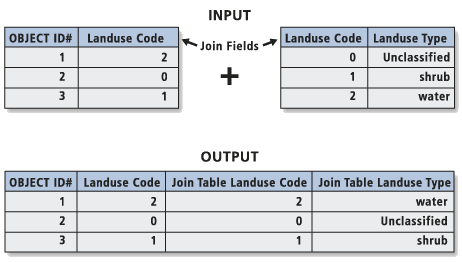
\includegraphics[width=0.8\linewidth]{../images/Join} \end{center}

\end{frame}

\begin{frame}[fragile]{Enriching Data: Example}

\begin{itemize}
\tightlist
\item
  Let's join some census data with shapefiles for the Southampton region
\end{itemize}

\begin{Shaded}
\begin{Highlighting}[]
\CommentTok{# Load Shapefile}
\NormalTok{Solent <-}\StringTok{ }\KeywordTok{readOGR}\NormalTok{(}\DataTypeTok{dsn =} \StringTok{"../data/SolentLEP"}\NormalTok{, }\StringTok{"Solent_revised"}\NormalTok{, }
    \DataTypeTok{verbose =} \OtherTok{FALSE}\NormalTok{)}
\KeywordTok{head}\NormalTok{(Solent[}\DecValTok{1}\NormalTok{:}\DecValTok{4}\NormalTok{], }\DataTypeTok{n =} \DecValTok{2}\NormalTok{)}
\end{Highlighting}
\end{Shaded}

\begin{verbatim}
##      OA11CD   LAD11CD LAD11NM  AREA_HECT
## 0 E00116566 E07000090  Havant 5.84000000
## 1 E00116564 E07000090  Havant 9.75000000
\end{verbatim}

\begin{Shaded}
\begin{Highlighting}[]
\KeywordTok{nrow}\NormalTok{(Solent)}
\end{Highlighting}
\end{Shaded}

\begin{verbatim}
## [1] 3826
\end{verbatim}

\end{frame}

\begin{frame}[fragile]{Enriching Data: Example}

\begin{itemize}
\tightlist
\item
  We can load some Census Data
\end{itemize}

\begin{Shaded}
\begin{Highlighting}[]
\CommentTok{# Age data for all of the UK}
\NormalTok{AgeData <-}\StringTok{ }\KeywordTok{read.csv}\NormalTok{(}\StringTok{"../data/MedianAge.csv"}\NormalTok{, }
                    \DataTypeTok{stringsAsFactors =} \OtherTok{FALSE}\NormalTok{)}
\KeywordTok{head}\NormalTok{(AgeData,}\DataTypeTok{n=}\DecValTok{3}\NormalTok{)}
\end{Highlighting}
\end{Shaded}

\begin{verbatim}
##   GeographyCode MedianAge
## 1     K04000001        39
## 2     E92000001        39
## 3     W92000004        41
\end{verbatim}

\begin{Shaded}
\begin{Highlighting}[]
\KeywordTok{nrow}\NormalTok{(AgeData)}
\end{Highlighting}
\end{Shaded}

\begin{verbatim}
## [1] 223722
\end{verbatim}

\begin{itemize}
\tightlist
\item
  The age data has records for the whole of England
\end{itemize}

\end{frame}

\begin{frame}[fragile]{Enriching Data: Example}

\begin{itemize}
\tightlist
\item
  We can easily merge the age data with the boundary data using the
  \texttt{merge()} function
\end{itemize}

\begin{Shaded}
\begin{Highlighting}[]
\CommentTok{# Merge Datasets}
\NormalTok{SolentMerged <-}\StringTok{ }\KeywordTok{merge}\NormalTok{(Solent, AgeData, }\DataTypeTok{by.x =} \StringTok{"OA11CD"}\NormalTok{, }
    \DataTypeTok{by.y =} \StringTok{"GeographyCode"}\NormalTok{)}
\CommentTok{# Lets focus on Southampton}
\NormalTok{Southampton <-}\StringTok{ }\NormalTok{SolentMerged[SolentMerged$LAD11NM ==}\StringTok{ }
\StringTok{    "Southampton"}\NormalTok{, ]}
\end{Highlighting}
\end{Shaded}

\end{frame}

\begin{frame}[fragile]{Enriching Data: Example}

\begin{Shaded}
\begin{Highlighting}[]
\KeywordTok{spplot}\NormalTok{(Southampton, }\StringTok{"MedianAge"}\NormalTok{, }\DataTypeTok{main =} \StringTok{"Median Age (years)"}\NormalTok{)}
\end{Highlighting}
\end{Shaded}

\begin{figure}

{\centering 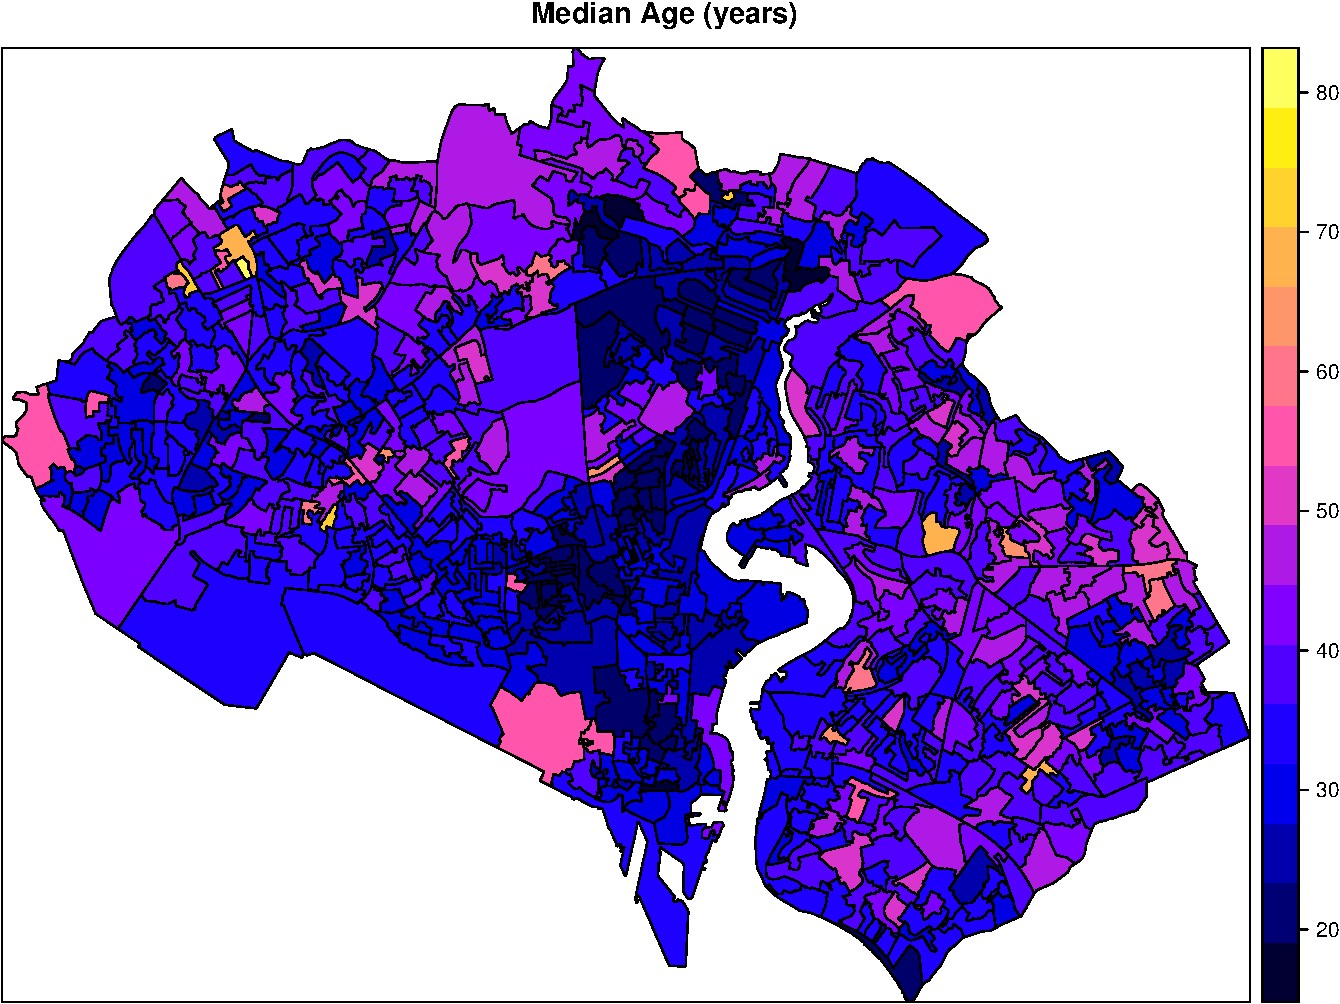
\includegraphics[width=0.7\linewidth]{SpatialDataLecture_files/figure-beamer/unnamed-chunk-24-1} 

}

\caption{Median Age with Output Areas in Southampton. Data from 2011 Census}\label{fig:unnamed-chunk-24}
\end{figure}

\end{frame}

\section{PART III: Coordinate Reference
Systems}\label{part-iii-coordinate-reference-systems}

\begin{frame}{Coordinate Reference Systems (CRS)}

\begincols
\begincol{.65\textwidth}

\begin{itemize}
\tightlist
\item
  Very important! R won't give you a warning when loading like in
  ArcGIS.
\item
  You don't always need to give one, but it is recommended to always do.
\item
  If you create spatial data, \textbf{you will usually have to specify}
  the projection.
\item
  packages \alert{sp} and \alert{rgdal} are used for managing CRS.
\end{itemize}

\endcol
\begincol{.34\textwidth}

\begin{center}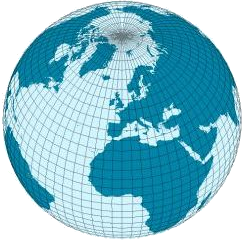
\includegraphics[width=0.5\linewidth]{../images/CRS} \end{center}

\endcol
\endcols

\begin{alertblock}{Find out more}
A useful guide is provided here about spatial projection in R \url{https://goo.gl/FAsv4k}
\end{alertblock}

\end{frame}

\begin{frame}[fragile]{Coordinate Systems: Example}

\begin{itemize}
\tightlist
\item
  Earlier, we created the SpatialDataFrame of Canadian Cities called
  \texttt{cities}.
\item
  We can check the spatial projection using the function \texttt{crs()}
\end{itemize}

\begin{Shaded}
\begin{Highlighting}[]
\KeywordTok{crs}\NormalTok{(cities)}
\end{Highlighting}
\end{Shaded}

\begin{verbatim}
## CRS arguments: NA
\end{verbatim}

\begin{itemize}
\tightlist
\item
  Currently the data has no CRS! We need to assign one
\item
  Dataset has WGS84 projection, which is the mostly commonly used
\end{itemize}

\begin{Shaded}
\begin{Highlighting}[]
\CommentTok{# Assign Projection to Cities}
\KeywordTok{crs}\NormalTok{(cities) <-}\StringTok{ }\KeywordTok{CRS}\NormalTok{(}\StringTok{"+init=epsg:4326"}\NormalTok{)}
\end{Highlighting}
\end{Shaded}

\begin{alertblock}{Find out spatial projection codes}
An online registry of spatial projections is available at \url{http://www.epsg-registry.org} for Coordinate Reference Systems
\end{alertblock}

\end{frame}

\begin{frame}[fragile]{Coordinate Systems: Example}

\begin{itemize}
\tightlist
\item
  We will load data for administrative borders in Canada using the
  function \texttt{getData()} from the \alert{raster} package
  \footnote<.->{This provides global vector and raster data for
    countries, administrative boundaries, altitude models and climatic
    data.}.
\end{itemize}

\begin{Shaded}
\begin{Highlighting}[]
\CommentTok{# Load Canada Data}
\NormalTok{canada <-}\StringTok{ }\NormalTok{raster::}\KeywordTok{getData}\NormalTok{(}\StringTok{"GADM"}\NormalTok{, }\DataTypeTok{country =} \StringTok{"CAN"}\NormalTok{, }
    \DataTypeTok{level =} \DecValTok{0}\NormalTok{, }\DataTypeTok{download =} \OtherTok{FALSE}\NormalTok{, }\DataTypeTok{path =} \StringTok{"../data"}\NormalTok{)}
\CommentTok{# Check Coordinate System}
\KeywordTok{crs}\NormalTok{(canada)}
\end{Highlighting}
\end{Shaded}

\begin{verbatim}
## CRS arguments:
##  +proj=longlat +datum=WGS84 +no_defs +ellps=WGS84 +towgs84=0,0,0
\end{verbatim}

\end{frame}

\begin{frame}{Coordinate Systems: Example}

\begin{center}\includegraphics[width=0.75\linewidth]{SpatialDataLecture_files/figure-beamer/unnamed-chunk-30-1} \end{center}

\end{frame}

\begin{frame}[fragile]{Example: Reprojecting}

\begin{itemize}
\tightlist
\item
  The function \texttt{spTransform()} can be used to reproject a CRS
\end{itemize}

\begin{Shaded}
\begin{Highlighting}[]
\NormalTok{GB <-}\StringTok{ }\NormalTok{raster::}\KeywordTok{getData}\NormalTok{(}\StringTok{"GADM"}\NormalTok{, }\DataTypeTok{country =} \StringTok{"GBR"}\NormalTok{, }\DataTypeTok{level =} \DecValTok{1}\NormalTok{, }
    \DataTypeTok{path =} \StringTok{"../data"}\NormalTok{)}
\NormalTok{GB_BNG <-}\StringTok{ }\KeywordTok{spTransform}\NormalTok{(GB, }\KeywordTok{CRS}\NormalTok{(}\StringTok{"+init=epsg:27700"}\NormalTok{))}
\end{Highlighting}
\end{Shaded}

\begin{figure}

{\centering 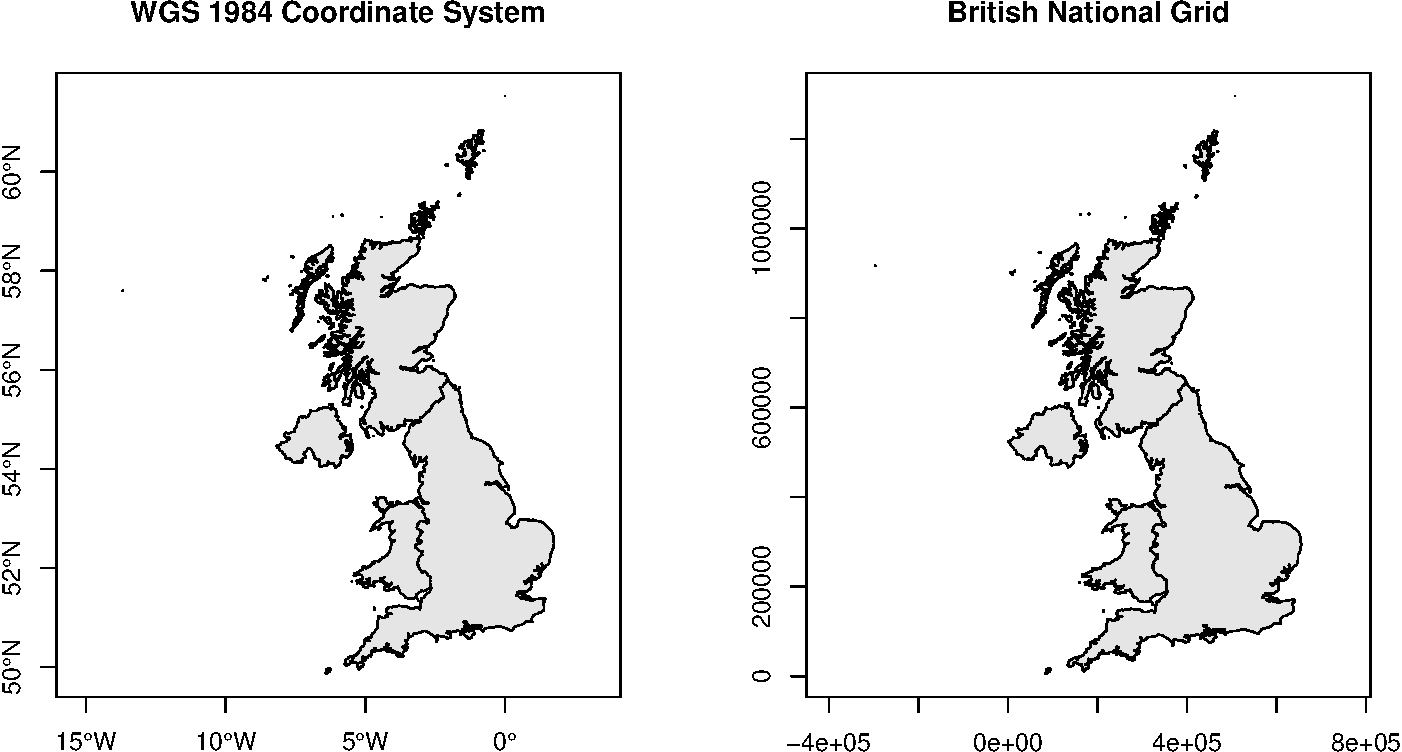
\includegraphics[width=0.8\linewidth]{SpatialDataLecture_files/figure-beamer/unnamed-chunk-32-1} 

}

\caption{Comparison of coordinate systems}\label{fig:unnamed-chunk-32}
\end{figure}

\end{frame}

\section{PART IV: Geoprocessing}\label{part-iv-geoprocessing}

\begin{frame}{Geoprocessing: rgeos package}

\begincols
\begincol{.69\textwidth}

\begin{itemize}
\tightlist
\item
  \alert{rgeos} is the main package used within R for geospatial
  analysis
\item
  interface to GEOS (Geometry Engine Open Source) Library
\end{itemize}

\endcol
\begincol{.3\textwidth}

\begin{center}
\includegraphics[width=0.8\linewidth]{../images/toolbox} \end{center}

\endcol
\endcols

\begin{alertblock}{Example Processes}
Union, distance, intersection, convex hull, envelope, buffer, simplify, polygon assembly, valid, area, length, intersects, touches, disjoint, crosses, within, contains, overlaps, equals, covers, etc.
\end{alertblock}

\end{frame}

\begin{frame}[fragile]{Buffer}

\begin{itemize}
\tightlist
\item
  apply a 2km buffer to the county of Inverness
\end{itemize}

\begin{Shaded}
\begin{Highlighting}[]
\NormalTok{inver <-}\StringTok{ }\NormalTok{scotland[scotland$NAME ==}\StringTok{ "Inverness"}\NormalTok{, ]}
\NormalTok{inver_buf <-}\StringTok{ }\KeywordTok{gBuffer}\NormalTok{(inver, }\DataTypeTok{width =} \DecValTok{2000}\NormalTok{)}
\end{Highlighting}
\end{Shaded}

\begin{center}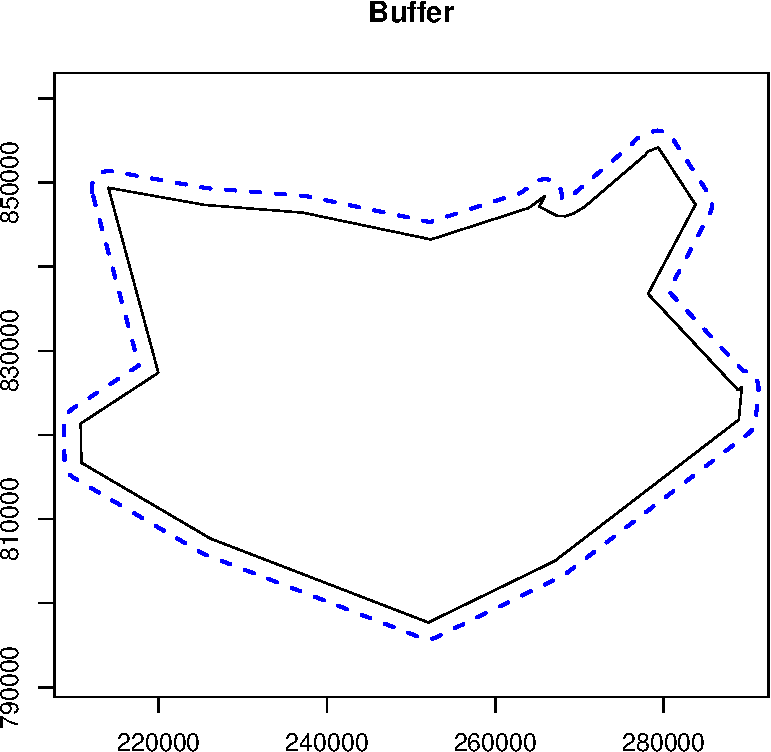
\includegraphics[width=0.5\linewidth]{SpatialDataLecture_files/figure-beamer/buf_inverness-1} \end{center}

\end{frame}

\begin{frame}[fragile]{Delaunay Triangulation}

\begin{itemize}
\tightlist
\item
  Form Delaunay triangulation for the cities in Canada
\end{itemize}

\begin{Shaded}
\begin{Highlighting}[]
\NormalTok{delTri <-}\StringTok{ }\KeywordTok{gDelaunayTriangulation}\NormalTok{(BigCities)}
\KeywordTok{plot}\NormalTok{(delTri, }\DataTypeTok{axes =} \OtherTok{TRUE}\NormalTok{, , }\DataTypeTok{main =} \StringTok{"Delaunay Triangulation"}\NormalTok{)}
\KeywordTok{plot}\NormalTok{(BigCities, }\DataTypeTok{col =} \StringTok{"red"}\NormalTok{, }\DataTypeTok{pch =} \DecValTok{16}\NormalTok{, }\DataTypeTok{cex =} \DecValTok{2}\NormalTok{, }\DataTypeTok{add =} \OtherTok{TRUE}\NormalTok{)}
\end{Highlighting}
\end{Shaded}

\begin{center}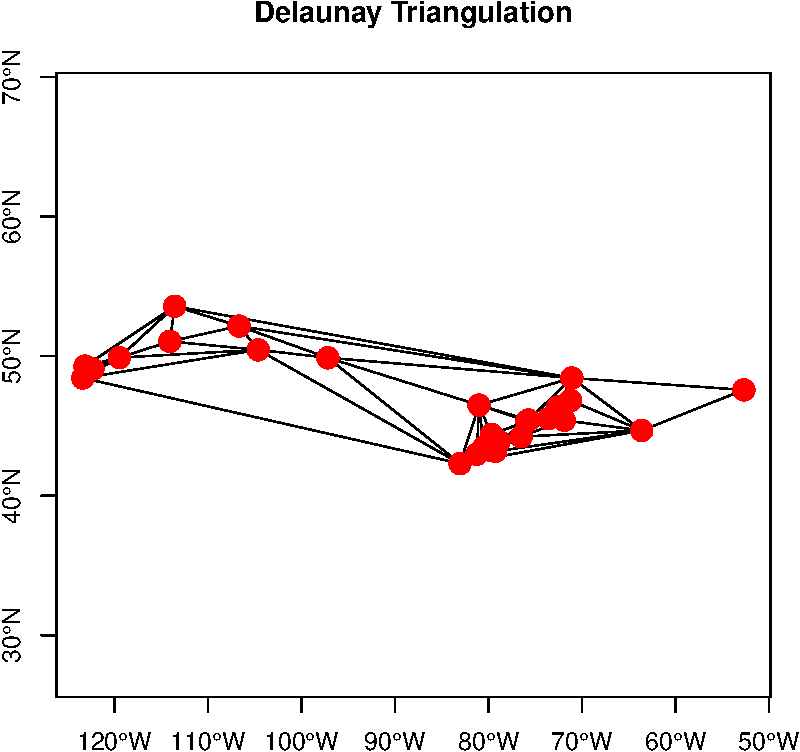
\includegraphics[width=0.5\linewidth]{SpatialDataLecture_files/figure-beamer/delaunay_tri-1} \end{center}

\end{frame}

\begin{frame}[fragile]{Spatial Proximity}

\begin{itemize}
\tightlist
\item
  How far is it to the nearest city?
\item
  \alert{spatstat} provides adds a spatial proximity functions.
\end{itemize}

\begin{Shaded}
\begin{Highlighting}[]
\KeywordTok{library}\NormalTok{(spatstat)}
\NormalTok{BigCities$Distance <-}\StringTok{ }\KeywordTok{nndist}\NormalTok{(}\DataTypeTok{X =} \NormalTok{BigCities@coords)}
\KeywordTok{spplot}\NormalTok{(BigCities, }\StringTok{"Distance"}\NormalTok{)  }\CommentTok{# Plot Results}
\end{Highlighting}
\end{Shaded}

\begin{center}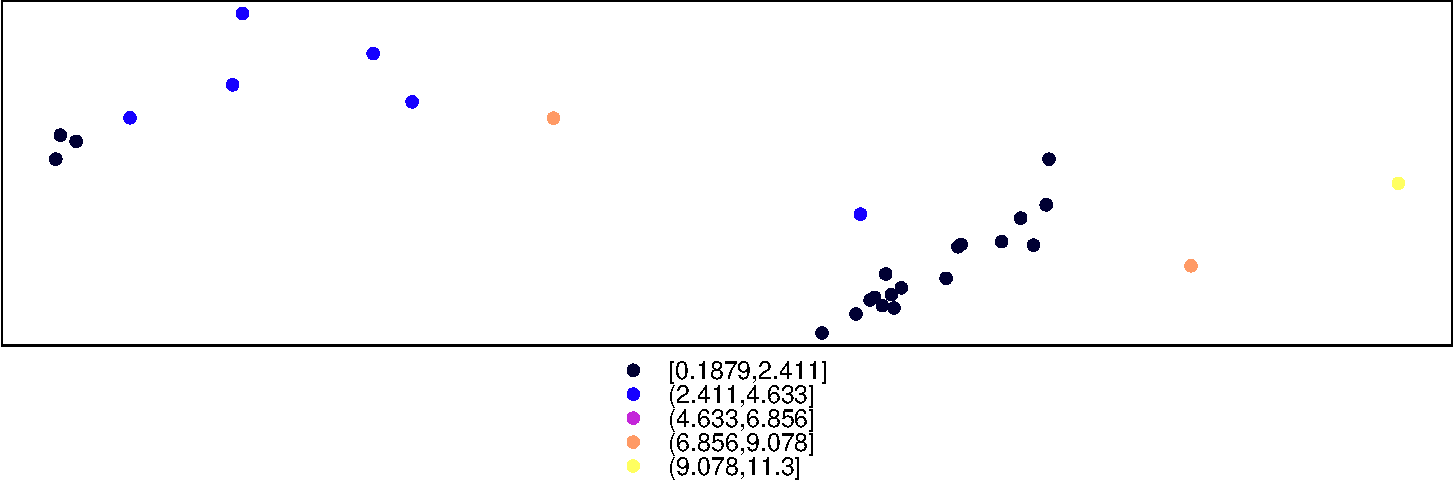
\includegraphics[width=0.8\linewidth]{SpatialDataLecture_files/figure-beamer/unnamed-chunk-35-1} \end{center}

\end{frame}

\section{PART V: Raster Data}\label{part-v-raster-data}

\begin{frame}[fragile]{Raster package}

\begincols
\begincol{.65\textwidth}

\begin{itemize}
\tightlist
\item
  Most control through \texttt{raster} package
\item
  Read, write and manipulate gridded spatial data
\item
  Basic and high-level analysis functions
\item
  Processing of large files
\end{itemize}

\endcol
\begincol{.34\textwidth}

\begin{center}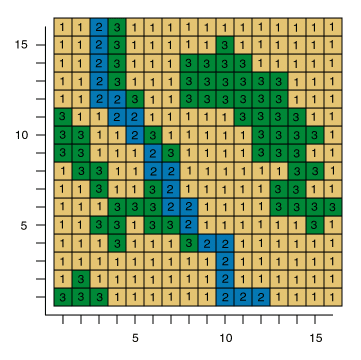
\includegraphics[width=1\linewidth]{../images/Raster} \end{center}

\endcol
\endcols

\end{frame}

\begin{frame}[fragile]{Raster Layer: Create from Scratch}

\begin{Shaded}
\begin{Highlighting}[]
\NormalTok{myrast <-}\StringTok{ }\KeywordTok{raster}\NormalTok{(}\KeywordTok{extent}\NormalTok{(}\KeywordTok{c}\NormalTok{(}\DecValTok{0}\NormalTok{, }\DecValTok{20}\NormalTok{, }\DecValTok{0}\NormalTok{, }\DecValTok{20}\NormalTok{)), }\DataTypeTok{ncol =} \DecValTok{10}\NormalTok{, }
    \DataTypeTok{nrow =} \DecValTok{10}\NormalTok{)}
\NormalTok{myrast[] <-}\StringTok{ }\DecValTok{1}\NormalTok{:}\DecValTok{100}
\NormalTok{myrast}
\end{Highlighting}
\end{Shaded}

\begin{verbatim}
## class       : RasterLayer 
## dimensions  : 10, 10, 100  (nrow, ncol, ncell)
## resolution  : 2, 2  (x, y)
## extent      : 0, 20, 0, 20  (xmin, xmax, ymin, ymax)
## coord. ref. : NA 
## data source : in memory
## names       : layer 
## values      : 1, 100  (min, max)
\end{verbatim}

\end{frame}

\begin{frame}[fragile]{Raster Layer: Raster Algebra}

\begin{itemize}
\tightlist
\item
  Rasters can be added, multiplied etc.
\end{itemize}

\begin{Shaded}
\begin{Highlighting}[]
\KeywordTok{par}\NormalTok{(}\DataTypeTok{mfrow =} \KeywordTok{c}\NormalTok{(}\DecValTok{1}\NormalTok{, }\DecValTok{2}\NormalTok{))  }\CommentTok{# Plot graphs side by side}
\KeywordTok{plot}\NormalTok{(myrast, }\DataTypeTok{main =} \StringTok{"Raster Value"}\NormalTok{, }\DataTypeTok{asp =} \DecValTok{1}\NormalTok{)}
\NormalTok{myrastSquared <-}\StringTok{ }\NormalTok{myrast^}\DecValTok{2}
\KeywordTok{plot}\NormalTok{(myrastSquared, }\DataTypeTok{main =} \StringTok{"Raster Value Squared"}\NormalTok{, }
    \DataTypeTok{asp =} \DecValTok{1}\NormalTok{)}
\end{Highlighting}
\end{Shaded}

\begin{center}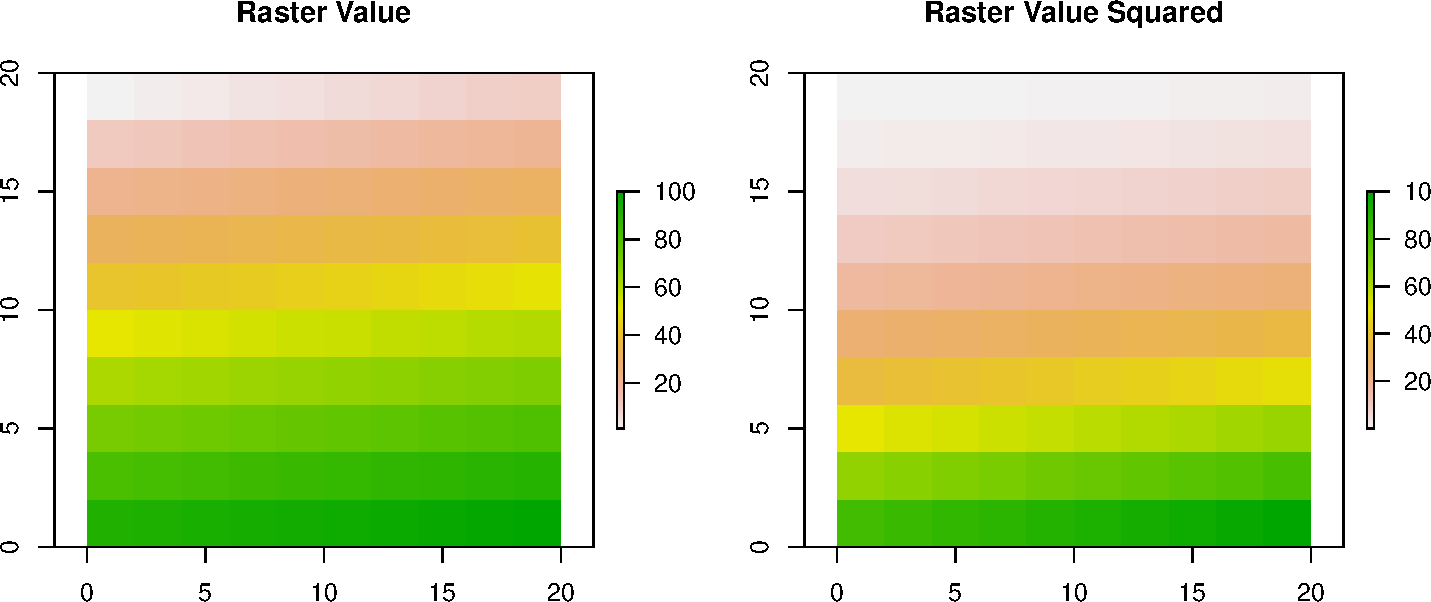
\includegraphics[width=0.8\linewidth]{SpatialDataLecture_files/figure-beamer/plot_rast01-1} \end{center}

\end{frame}

\begin{frame}[fragile]{Raster Data: Import a GeoTiff}

\begin{itemize}
\tightlist
\item
  The \texttt{raster()} function from the \alert{raster} package can be
  used
\end{itemize}

\begin{Shaded}
\begin{Highlighting}[]
\NormalTok{WindSpeedRaster <-}\StringTok{ }\KeywordTok{raster}\NormalTok{(}\DataTypeTok{x =} \StringTok{"../data/WindSpeed45.tif"}\NormalTok{)}
\KeywordTok{plot}\NormalTok{(WindSpeedRaster, }\StringTok{"WindSpeed45"}\NormalTok{)}
\end{Highlighting}
\end{Shaded}

\begin{figure}

{\centering 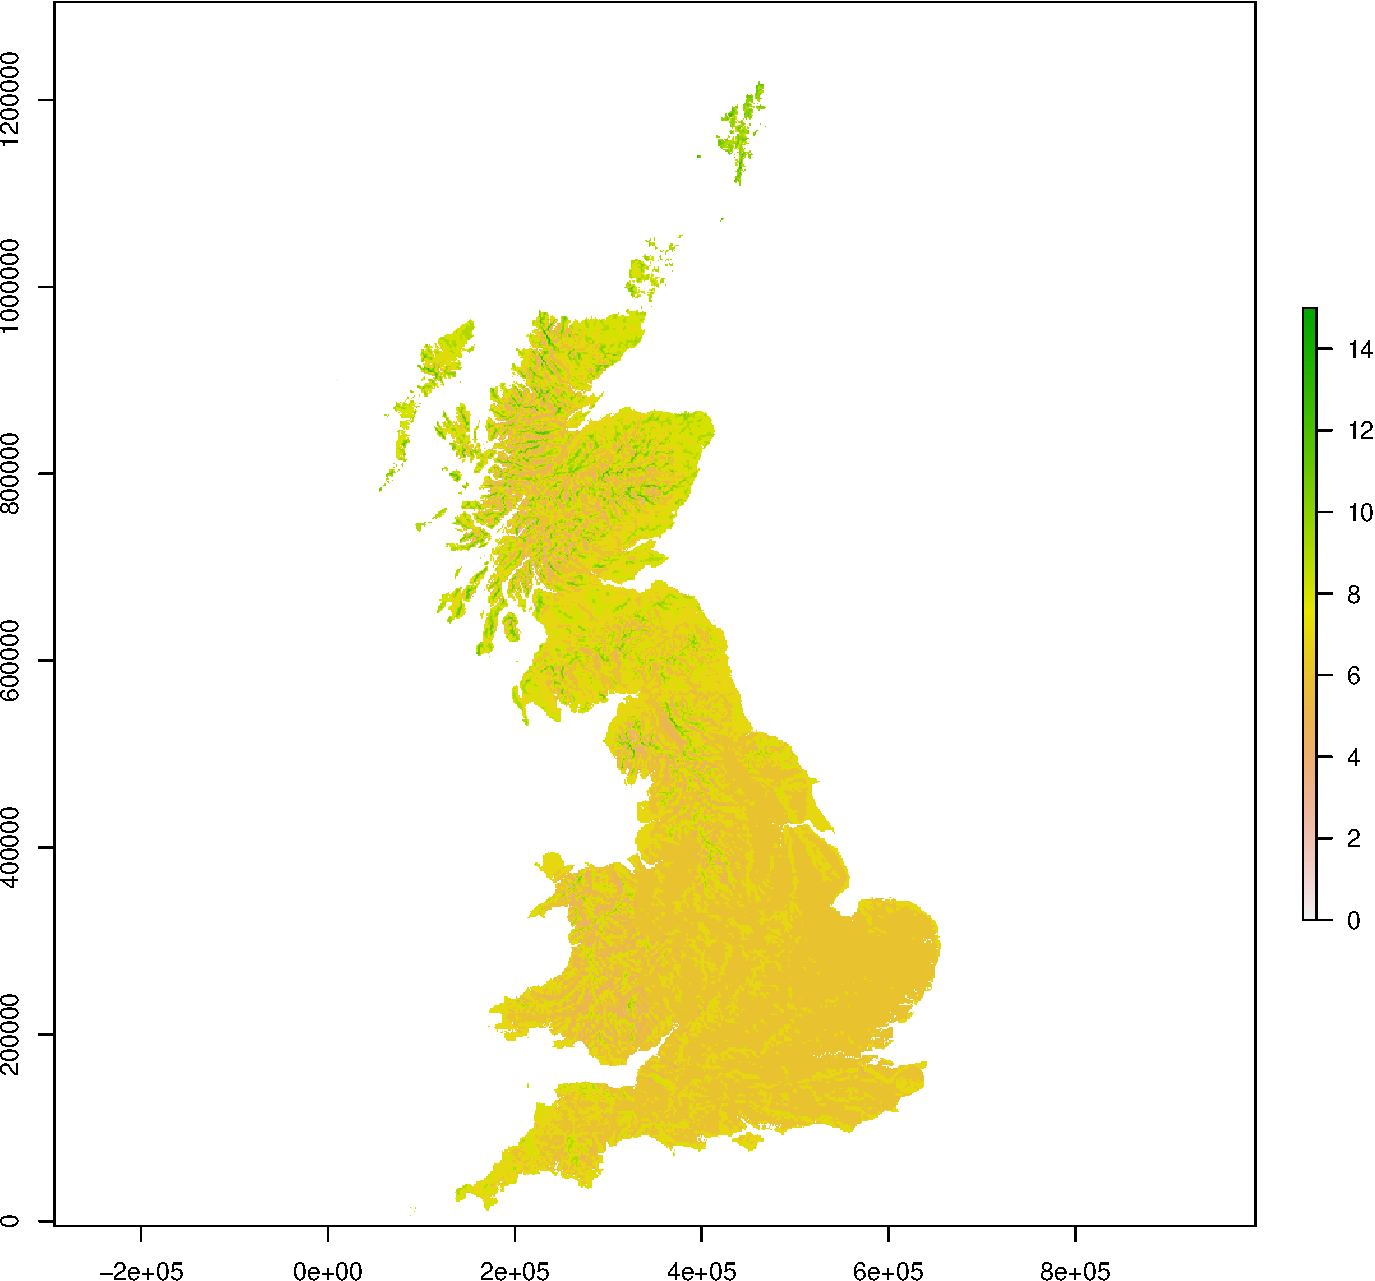
\includegraphics[width=0.6\linewidth]{SpatialDataLecture_files/figure-beamer/get_rasterdir_pictures-1} 

}

\caption{UK Annualised Wind Speed Map at 45m above ground level}\label{fig:get_rasterdir_pictures}
\end{figure}

\end{frame}

\begin{frame}[fragile]{Raster Data: Crop a Raster}

\begin{itemize}
\tightlist
\item
  \texttt{crop()} function can be used to clip a raster to a spatial
  extent
\end{itemize}

\begin{Shaded}
\begin{Highlighting}[]
\NormalTok{WindSpeedSolent <-}\StringTok{ }\KeywordTok{crop}\NormalTok{(WindSpeedRaster, Solent)}
\KeywordTok{plot}\NormalTok{(WindSpeedSolent, }\DataTypeTok{asp =} \DecValTok{1}\NormalTok{)}
\end{Highlighting}
\end{Shaded}

\begin{center}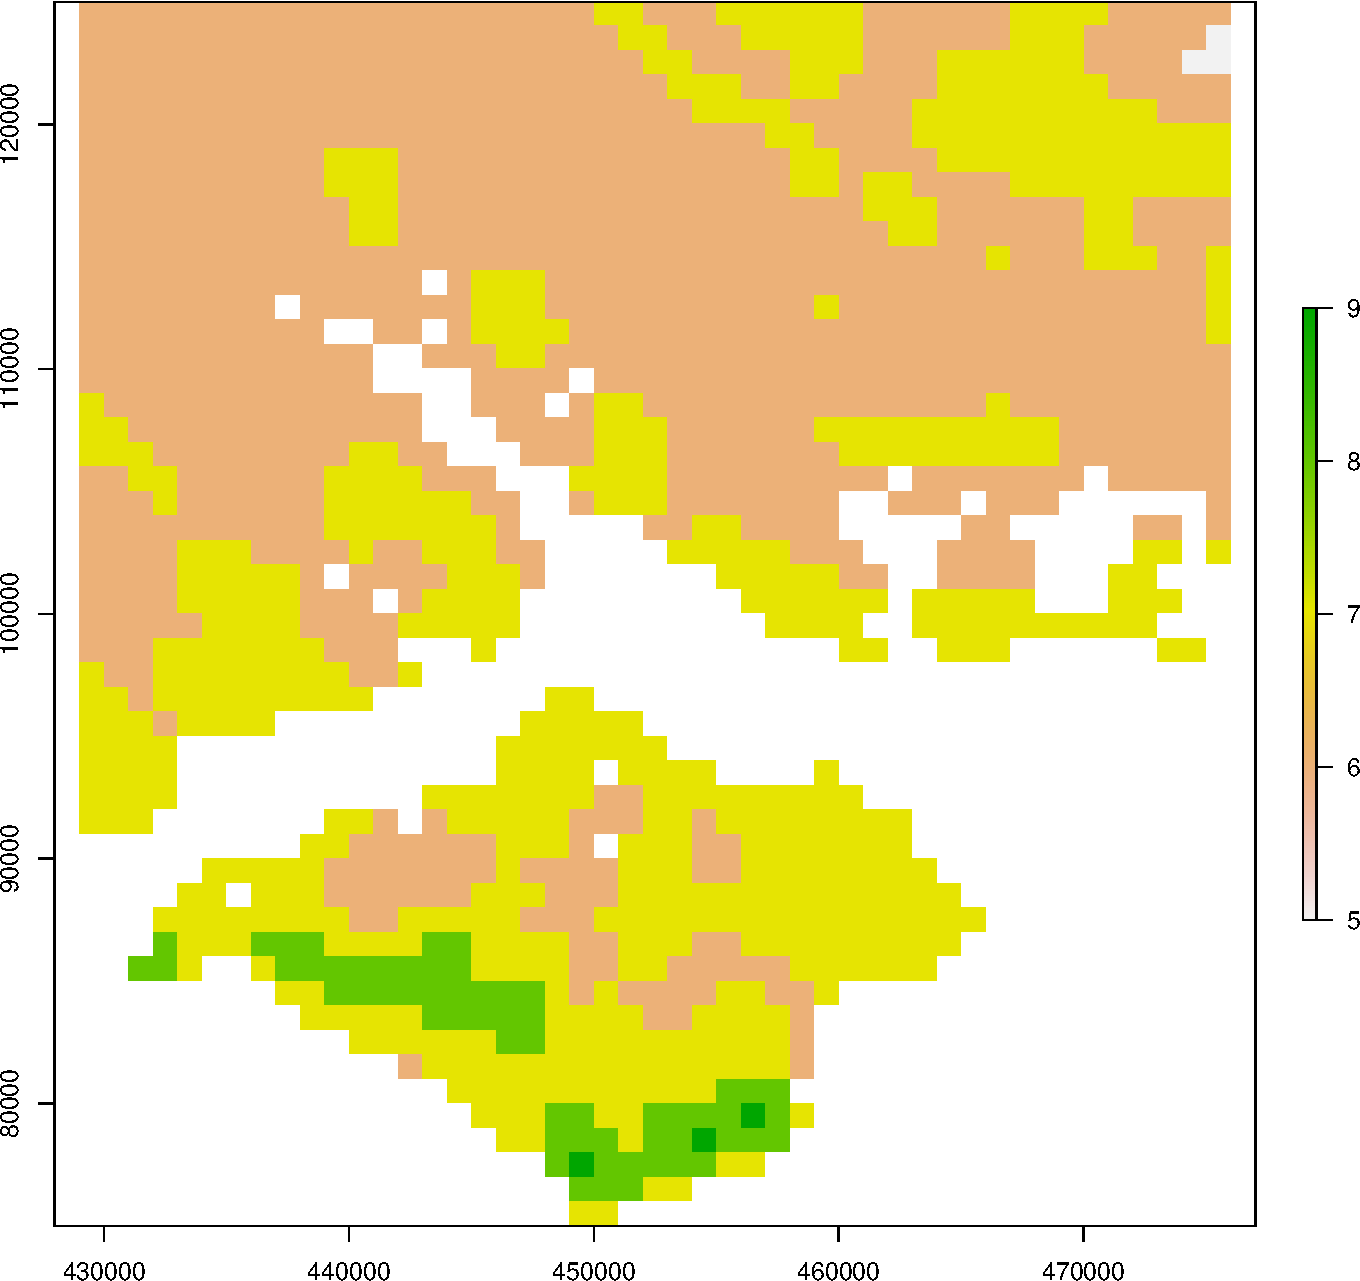
\includegraphics[width=0.45\linewidth]{SpatialDataLecture_files/figure-beamer/crop_peru_rast-1} \end{center}

\end{frame}

\begin{frame}[fragile]{Overlay Points and Extract Values}

\begin{itemize}
\tightlist
\item
  Generate Some Points Within The Solent Region
\item
  The \texttt{spsample()} function from the package \alert{sp} can to
  produce a sample within a given extent
\end{itemize}

\begin{Shaded}
\begin{Highlighting}[]
\NormalTok{SolentPoints <-}\StringTok{ }\KeywordTok{spsample}\NormalTok{(Solent, }\DataTypeTok{n =} \DecValTok{25}\NormalTok{, }\DataTypeTok{type =} \StringTok{"random"}\NormalTok{)}
\NormalTok{SolentPoints$ID <-}\StringTok{ }\DecValTok{1}\NormalTok{:}\KeywordTok{nrow}\NormalTok{(SolentPoints@coords)}
\end{Highlighting}
\end{Shaded}

\begin{center}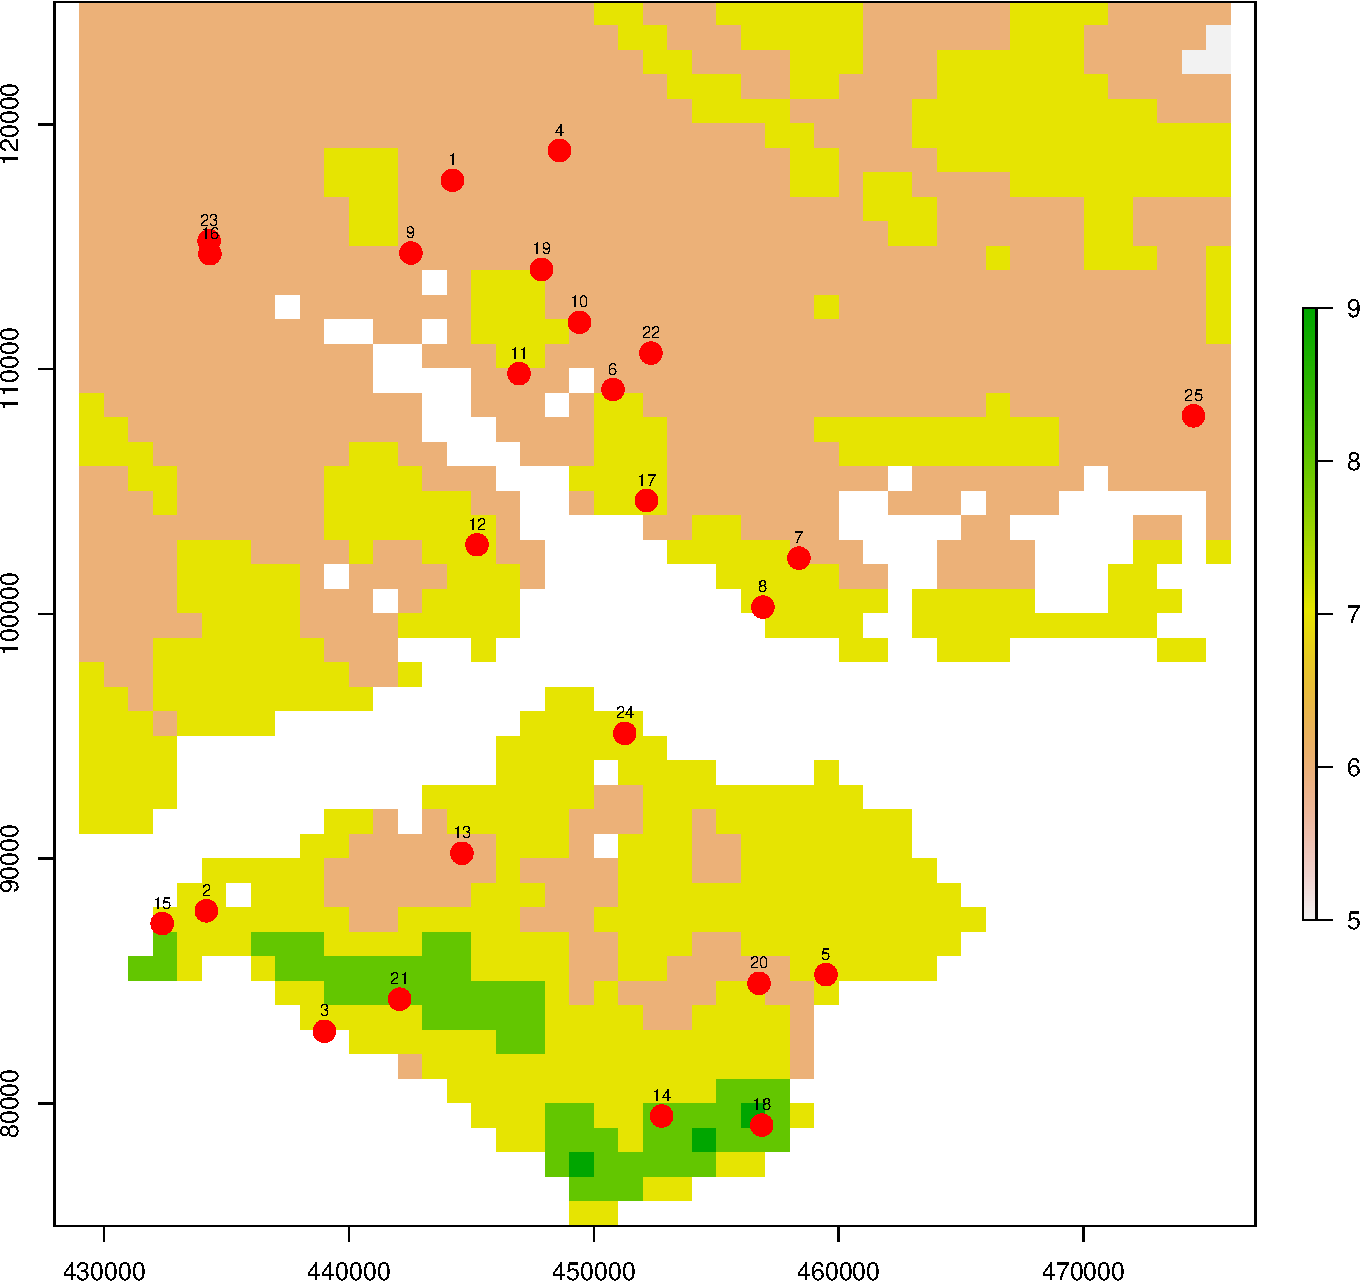
\includegraphics[width=0.5\linewidth]{SpatialDataLecture_files/figure-beamer/extract_vals_at_pts01-1} \end{center}

\end{frame}

\begin{frame}[fragile]{Overlay Points and Extract Values}

\begin{itemize}
\tightlist
\item
  You can use the \texttt{extract()} function to calculate the value at
  points.
\end{itemize}

\begin{Shaded}
\begin{Highlighting}[]
\KeywordTok{extract}\NormalTok{(WindSpeedSolent, SolentPoints)}
\end{Highlighting}
\end{Shaded}

\begin{verbatim}
##  [1]  6  7 NA  6  7  6  6  7  6  6  6  7  6  8  7  6  7  9  6  7  8  6  6
## [24]  7  6
\end{verbatim}

\end{frame}

\begin{frame}[fragile]{Create a Distance Surface}

\begin{itemize}
\tightlist
\item
  The function \texttt{distance()} can produce a proximity raster to the
  nearest spatial point
\item
  We must first \texttt{rasterize()} the Vector data (SpatialPoints)
\end{itemize}

\begin{Shaded}
\begin{Highlighting}[]
\NormalTok{SolentPointsRast <-}\StringTok{ }\KeywordTok{rasterize}\NormalTok{(SolentPoints, WindSpeedSolent, }
    \DataTypeTok{field =} \DecValTok{1}\NormalTok{)}
\NormalTok{dist2SamplePtsRast <-}\StringTok{ }\KeywordTok{distance}\NormalTok{(SolentPointsRast)}
\end{Highlighting}
\end{Shaded}

\begin{center}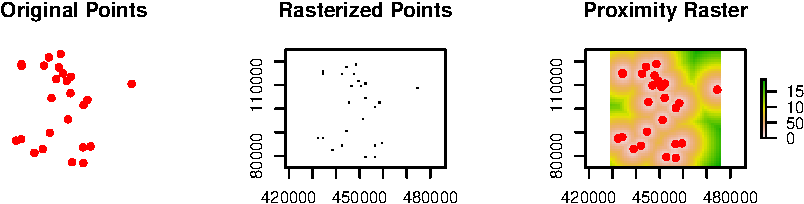
\includegraphics[width=1\linewidth]{SpatialDataLecture_files/figure-beamer/unnamed-chunk-38-1} \end{center}

\end{frame}

\section{PART VI: Displaying Results}\label{part-vi-displaying-results}

\begin{frame}[fragile]{ggplot: the basics}

\begincols
\begincol{.48\textwidth}

\begin{itemize}
\tightlist
\item
  Maps so far have been quite basic and produced with the functions
  \texttt{plot()} or \texttt{spplot()}
\item
  Easy to produce, but not the most attractive
\item
  Time to use \alert{ggplot2}
\item
  Same procedure as building graphs, with a few minor differences
\end{itemize}

\endcol
\begincol{.48\textwidth}

\begin{center}
\includegraphics[width=1\linewidth]{../images/ggplot} \end{center}

\endcol
\endcols

\begin{alertblock}{Warning}
Don't worry if you don't understand all the examples. They can be used for future reference.
\end{alertblock}

\end{frame}

\begin{frame}{ggplot Example: A World Map}

\begin{itemize}
\tightlist
\item
  Places I have visited.
\end{itemize}

\begin{center}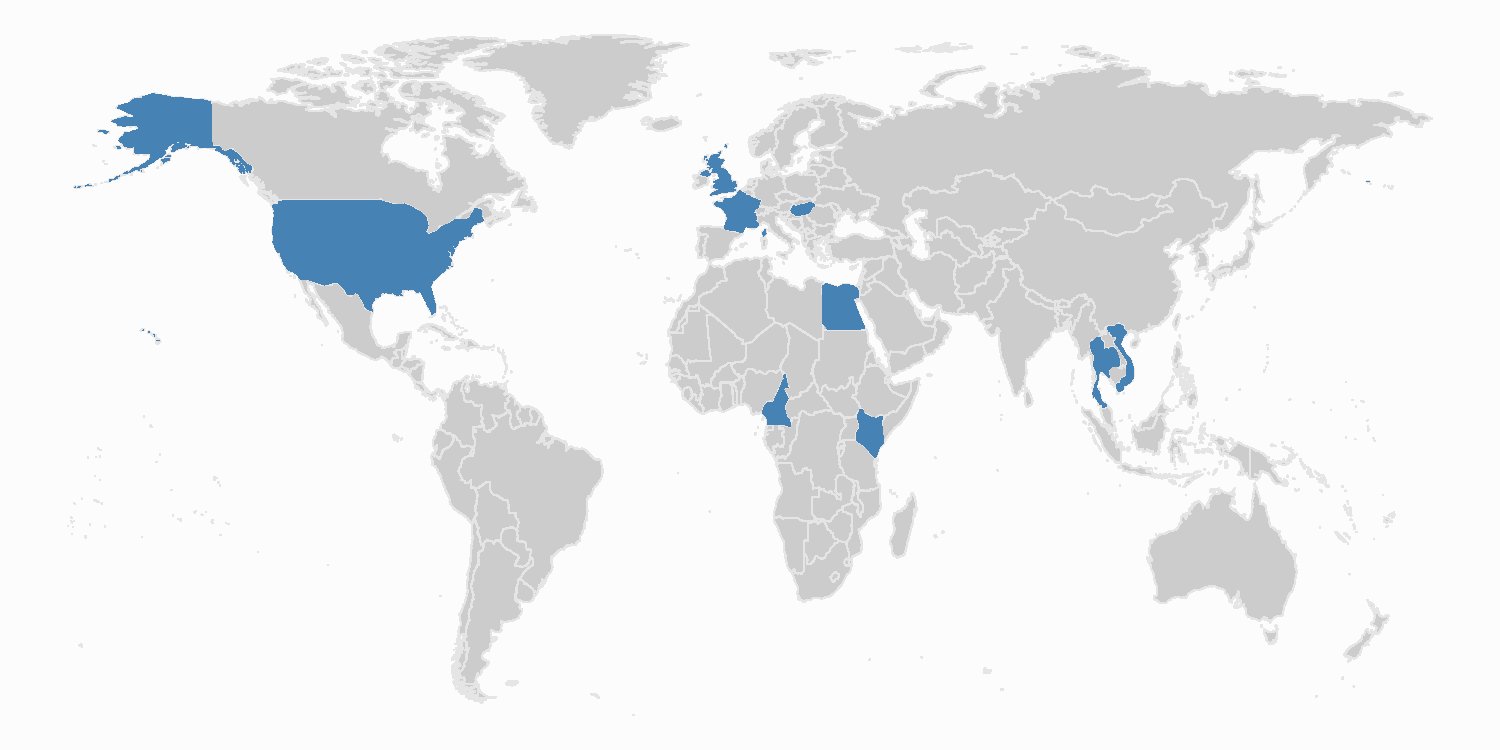
\includegraphics[width=1\linewidth]{SpatialDataLecture_files/figure-beamer/unnamed-chunk-40-1} \end{center}

\end{frame}

\begin{frame}[fragile]{ggplot Example: A World Map}

\begin{itemize}
\tightlist
\item
  Map made with less than 15 lines of code.
\end{itemize}

\tiny

\begin{Shaded}
\begin{Highlighting}[]
\KeywordTok{library}\NormalTok{(mapdata)}
\KeywordTok{library}\NormalTok{(ggmap)}

\CommentTok{# Load Data and select countries}
\NormalTok{World <-}\StringTok{ }\KeywordTok{map_data}\NormalTok{(}\DataTypeTok{map =} \StringTok{"world"}\NormalTok{)}
\NormalTok{World <-}\StringTok{ }\NormalTok{World[World$region !=}\StringTok{ "Antarctica"}\NormalTok{, ] }\CommentTok{# Remove Antartica as it looks bad on the map}

\CommentTok{# Select Highlight Regions}
\NormalTok{StudyRegions <-}\StringTok{ }\NormalTok{World[World$region ==}\StringTok{ }\KeywordTok{c}\NormalTok{(}\StringTok{"UK"}\NormalTok{, }\StringTok{"USA"}\NormalTok{, }\StringTok{"UAE"}\NormalTok{, }\StringTok{"Egypt"}\NormalTok{, }\StringTok{"Kenya"}\NormalTok{, }\StringTok{"Cameroon"}\NormalTok{,}
                                        \StringTok{"Hungary"}\NormalTok{, }\StringTok{"France"}\NormalTok{, }\StringTok{"Thailand"}\NormalTok{, }\StringTok{"Vietnam"}\NormalTok{),]}

\KeywordTok{ggplot}\NormalTok{() +}\StringTok{ }
\StringTok{  }\CommentTok{# Add the basemap}
\StringTok{  }\KeywordTok{geom_polygon}\NormalTok{(}\DataTypeTok{data =} \NormalTok{World, }\KeywordTok{aes}\NormalTok{(}\DataTypeTok{x=}\NormalTok{long, }\DataTypeTok{y =} \NormalTok{lat, }\DataTypeTok{group =} \NormalTok{group), }\DataTypeTok{fill =} \StringTok{"grey80"}\NormalTok{, }\DataTypeTok{colour =} \StringTok{"grey90"}\NormalTok{, }\DataTypeTok{size =} \FloatTok{0.25}\NormalTok{) +}\StringTok{ }
\StringTok{  }
\StringTok{  }\CommentTok{# Add the higlihhted Countries}
\StringTok{  }\KeywordTok{geom_polygon}\NormalTok{(}\DataTypeTok{data =} \NormalTok{StudyRegions, }\KeywordTok{aes}\NormalTok{(}\DataTypeTok{x=}\NormalTok{long, }\DataTypeTok{y =} \NormalTok{lat, }\DataTypeTok{group =} \NormalTok{group), }\DataTypeTok{fill =} \StringTok{"steelblue"}\NormalTok{) +}
\StringTok{  }
\StringTok{  }\CommentTok{# Coordinates}
\StringTok{    }\KeywordTok{coord_fixed}\NormalTok{(}\FloatTok{1.3}\NormalTok{) +}
\StringTok{  }
\StringTok{  }\CommentTok{# Themes}
\StringTok{  }\KeywordTok{theme_nothing}\NormalTok{() +}\StringTok{ }
\StringTok{  }\KeywordTok{theme}\NormalTok{(}\DataTypeTok{panel.background =} \KeywordTok{element_rect}\NormalTok{(}\DataTypeTok{fill =} \StringTok{'gray99'}\NormalTok{),}
        \DataTypeTok{plot.margin =} \KeywordTok{unit}\NormalTok{(}\KeywordTok{c}\NormalTok{(}\DecValTok{0}\NormalTok{,}\DecValTok{0}\NormalTok{,}\DecValTok{0}\NormalTok{,}\DecValTok{0}\NormalTok{), }\StringTok{"cm"}\NormalTok{))}
\end{Highlighting}
\end{Shaded}

\normalsize

\end{frame}

\begin{frame}{ggplot Examples: a choropleth map}

Another example from:
\url{http://docs.ggplot2.org/current/geom_map.html}

\begin{center}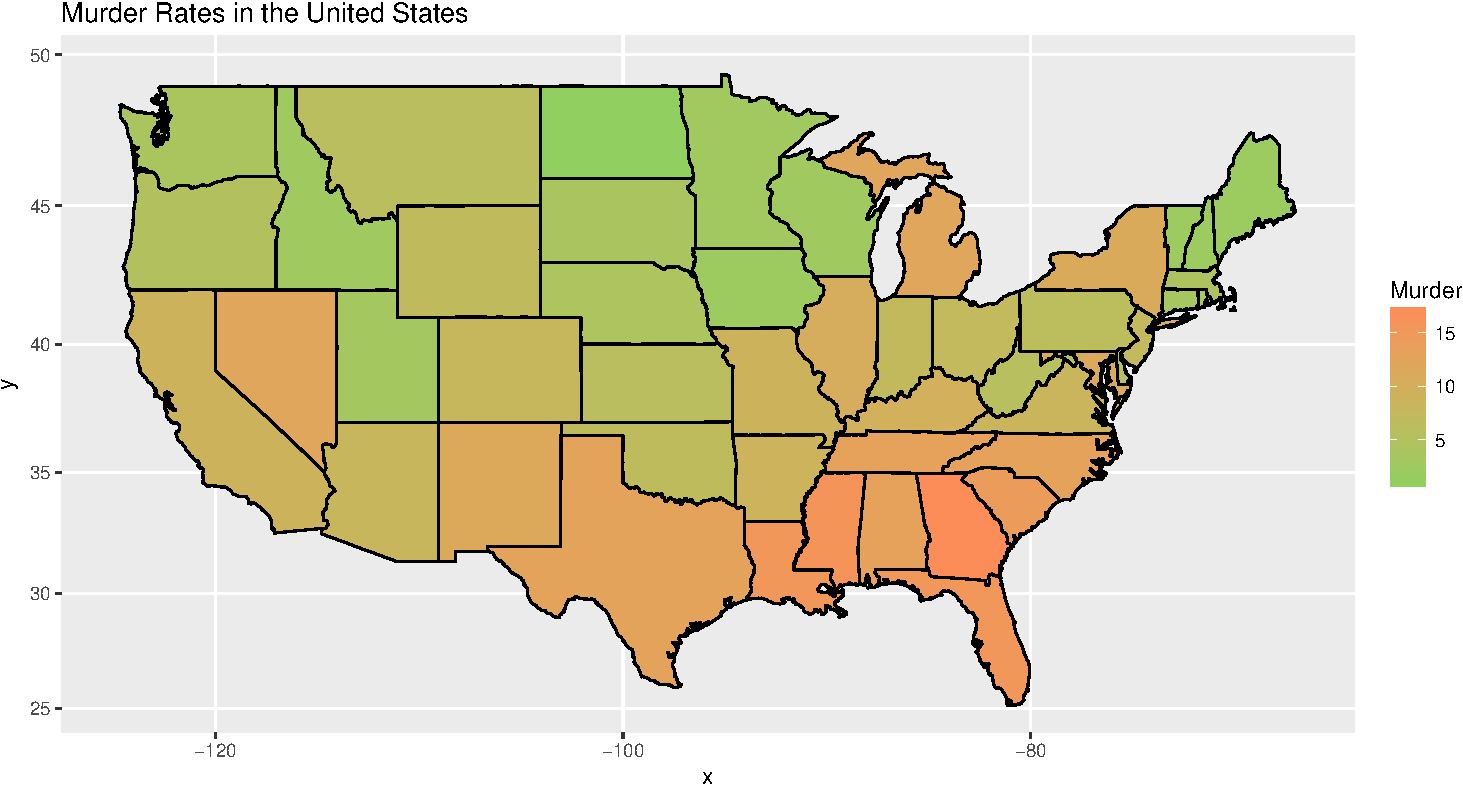
\includegraphics[width=1\linewidth]{SpatialDataLecture_files/figure-beamer/unnamed-chunk-42-1} \end{center}

\end{frame}

\begin{frame}{ggplot Examples: a faceted map}

\begin{center}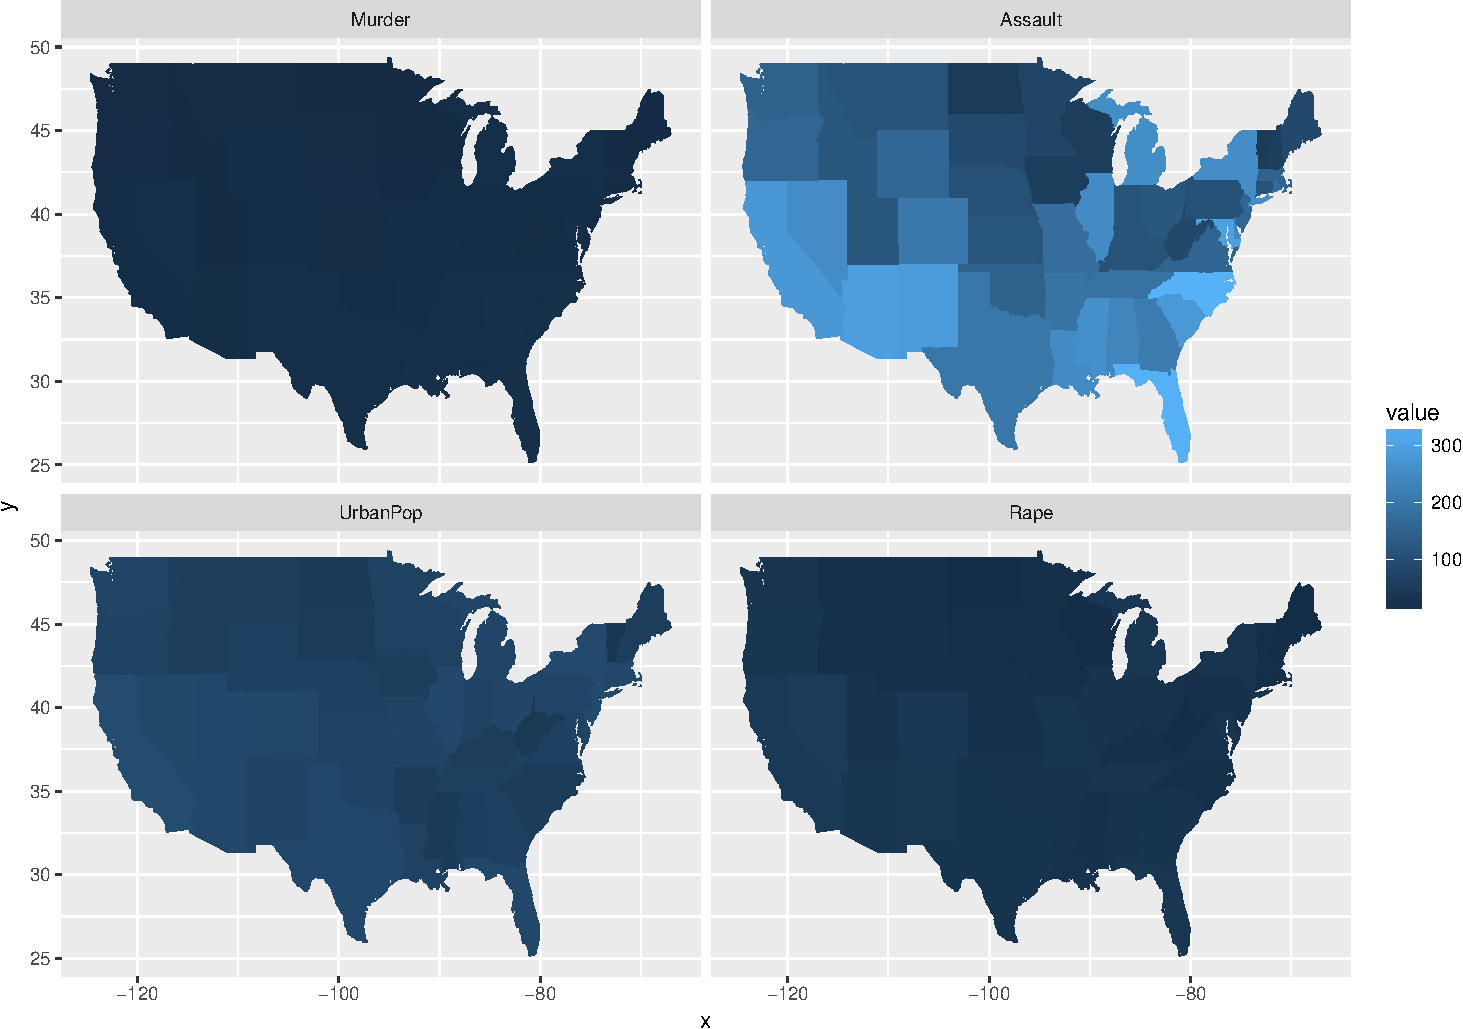
\includegraphics[width=1\linewidth]{SpatialDataLecture_files/figure-beamer/unnamed-chunk-43-1} \end{center}

\end{frame}

\begin{frame}[fragile]{ggplot Examples: a choropleth map}

\tiny

\begin{Shaded}
\begin{Highlighting}[]
\KeywordTok{library}\NormalTok{(ggplot2)}
\NormalTok{crimes <-}\StringTok{ }\KeywordTok{data.frame}\NormalTok{(}\DataTypeTok{state =} \KeywordTok{tolower}\NormalTok{(}\KeywordTok{rownames}\NormalTok{(USArrests)), }
    \NormalTok{USArrests)}
\KeywordTok{library}\NormalTok{(reshape2)  }\CommentTok{# for melt}
\NormalTok{crimesm <-}\StringTok{ }\KeywordTok{melt}\NormalTok{(crimes, }\DataTypeTok{id =} \DecValTok{1}\NormalTok{)}
\KeywordTok{library}\NormalTok{(maps)}

\NormalTok{states_map <-}\StringTok{ }\KeywordTok{map_data}\NormalTok{(}\StringTok{"state"}\NormalTok{)}

\CommentTok{# Murder Map}

\CommentTok{# Data & Aesthetics}
\KeywordTok{ggplot}\NormalTok{(crimes, }\KeywordTok{aes}\NormalTok{(}\DataTypeTok{map_id =} \NormalTok{state, }\DataTypeTok{fill =} \NormalTok{Murder)) +}\StringTok{ }
\StringTok{    }
\CommentTok{# Geometries}
\KeywordTok{geom_map}\NormalTok{(}\KeywordTok{aes}\NormalTok{(}\DataTypeTok{fill =} \NormalTok{Murder), }\DataTypeTok{map =} \NormalTok{states_map, }\DataTypeTok{colour =} \StringTok{"black"}\NormalTok{) +}\StringTok{ }
\StringTok{    }
\KeywordTok{scale_fill_gradient}\NormalTok{(}\DataTypeTok{low =} \StringTok{"#91cf60"}\NormalTok{, }\DataTypeTok{high =} \StringTok{"#fc8d59"}\NormalTok{) +}\StringTok{ }
\StringTok{    }
\CommentTok{# Coordinates}
\KeywordTok{expand_limits}\NormalTok{(}\DataTypeTok{x =} \NormalTok{states_map$long, }\DataTypeTok{y =} \NormalTok{states_map$lat) +}\StringTok{ }
\StringTok{    }\KeywordTok{coord_map}\NormalTok{() +}\StringTok{ }
\CommentTok{# Theme}
\KeywordTok{ggtitle}\NormalTok{(}\StringTok{"Murder Rates in the United States"}\NormalTok{)}


\CommentTok{# Faceted Map}
\KeywordTok{ggplot}\NormalTok{(crimesm, }\KeywordTok{aes}\NormalTok{(}\DataTypeTok{map_id =} \NormalTok{state)) +}\StringTok{ }\KeywordTok{geom_map}\NormalTok{(}\KeywordTok{aes}\NormalTok{(}\DataTypeTok{fill =} \NormalTok{value), }
    \DataTypeTok{map =} \NormalTok{states_map) +}\StringTok{ }\KeywordTok{expand_limits}\NormalTok{(}\DataTypeTok{x =} \NormalTok{states_map$long, }
    \DataTypeTok{y =} \NormalTok{states_map$lat) +}\StringTok{ }\KeywordTok{facet_wrap}\NormalTok{(~variable)}
\end{Highlighting}
\end{Shaded}

\normalsize

\end{frame}

\begin{frame}{ggplot Examples: spatial Points}

\begin{center}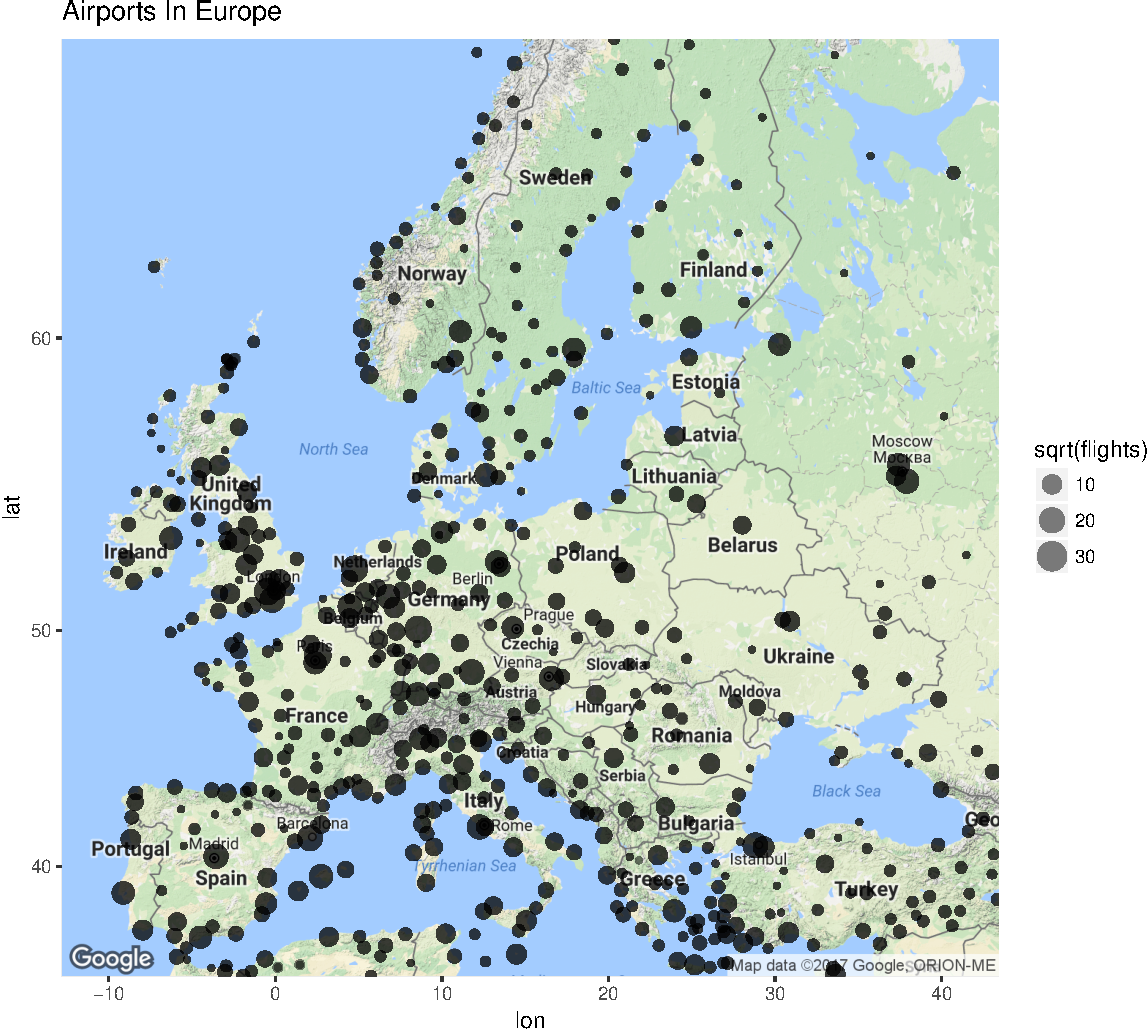
\includegraphics[width=0.8\linewidth]{SpatialDataLecture_files/figure-beamer/unnamed-chunk-45-1} \end{center}

\end{frame}

\begin{frame}[fragile]{ggplot Examples: spatial Points}

\tiny

\begin{Shaded}
\begin{Highlighting}[]
\CommentTok{#data}
\NormalTok{airports <-}\StringTok{ }\KeywordTok{read.csv}\NormalTok{(}\StringTok{"https://raw.githubusercontent.com/jpatokal/openflights/master/data/airports.dat"}\NormalTok{, }\DataTypeTok{header =} \OtherTok{FALSE}\NormalTok{)}
\KeywordTok{colnames}\NormalTok{(airports) <-}\StringTok{ }\KeywordTok{c}\NormalTok{(}\StringTok{"ID"}\NormalTok{, }\StringTok{"name"}\NormalTok{, }\StringTok{"city"}\NormalTok{, }\StringTok{"country"}\NormalTok{, }\StringTok{"IATA_FAA"}\NormalTok{, }\StringTok{"ICAO"}\NormalTok{, }\StringTok{"lat"}\NormalTok{, }\StringTok{"lon"}\NormalTok{, }\StringTok{"altitude"}\NormalTok{, }\StringTok{"timezone"}\NormalTok{, }\StringTok{"DST"}\NormalTok{)}
\NormalTok{routes <-}\StringTok{ }\KeywordTok{read.csv}\NormalTok{(}\StringTok{"https://raw.githubusercontent.com/jpatokal/openflights/master/data/routes.dat"}\NormalTok{, }\DataTypeTok{header=}\NormalTok{F)}
\KeywordTok{colnames}\NormalTok{(routes) <-}\StringTok{ }\KeywordTok{c}\NormalTok{(}\StringTok{"airline"}\NormalTok{, }\StringTok{"airlineID"}\NormalTok{, }\StringTok{"sourceAirport"}\NormalTok{, }\StringTok{"sourceAirportID"}\NormalTok{, }\StringTok{"destinationAirport"}\NormalTok{, }
                      \StringTok{"destinationAirportID"}\NormalTok{, }\StringTok{"codeshare"}\NormalTok{, }\StringTok{"stops"}\NormalTok{, }\StringTok{"equipment"}\NormalTok{)}

\KeywordTok{library}\NormalTok{(plyr)}
\NormalTok{departures <-}\StringTok{ }\KeywordTok{ddply}\NormalTok{(routes, .(sourceAirportID), }\StringTok{"nrow"}\NormalTok{)}
\KeywordTok{names}\NormalTok{(departures)[}\DecValTok{2}\NormalTok{] <-}\StringTok{ "flights"}
\NormalTok{arrivals <-}\StringTok{ }\KeywordTok{ddply}\NormalTok{(routes, .(destinationAirportID), }\StringTok{"nrow"}\NormalTok{)}
\KeywordTok{names}\NormalTok{(arrivals)[}\DecValTok{2}\NormalTok{] <-}\StringTok{ "flights"}

\NormalTok{airportD <-}\StringTok{ }\KeywordTok{merge}\NormalTok{(airports, departures, }\DataTypeTok{by.x =} \StringTok{"ID"}\NormalTok{, }\DataTypeTok{by.y =} \StringTok{"sourceAirportID"}\NormalTok{)}
\NormalTok{airportA <-}\StringTok{ }\KeywordTok{merge}\NormalTok{(airports, arrivals, }\DataTypeTok{by.x =} \StringTok{"ID"}\NormalTok{, }\DataTypeTok{by.y =} \StringTok{"destinationAirportID"}\NormalTok{)}

\NormalTok{map <-}\StringTok{ }\KeywordTok{get_map}\NormalTok{(}\DataTypeTok{location =} \StringTok{'Europe'}\NormalTok{, }\DataTypeTok{zoom =} \DecValTok{4}\NormalTok{, }\DataTypeTok{messaging =} \OtherTok{FALSE}\NormalTok{)}

\CommentTok{# create the data set containing both departures and arrivals}
\NormalTok{airportD$type <-}\StringTok{ "departures"}
\NormalTok{airportA$type <-}\StringTok{ "arrivals"}
\NormalTok{airportDA <-}\StringTok{ }\KeywordTok{rbind}\NormalTok{(airportD, airportA)}

\KeywordTok{ggmap}\NormalTok{(map) +}
\StringTok{  }\KeywordTok{geom_point}\NormalTok{(}\KeywordTok{aes}\NormalTok{(}\DataTypeTok{x =} \NormalTok{lon, }\DataTypeTok{y =} \NormalTok{lat, }\DataTypeTok{size =} \KeywordTok{sqrt}\NormalTok{(flights)), }\DataTypeTok{data =} \NormalTok{airportDA, }\DataTypeTok{alpha =} \NormalTok{.}\DecValTok{5}\NormalTok{) +}
\CommentTok{# panels according to type (departure/arrival) +}
\StringTok{  }\KeywordTok{ggtitle}\NormalTok{(}\StringTok{"Airports In Europe"}\NormalTok{) +}
\StringTok{  }\KeywordTok{guides}\NormalTok{(}\DataTypeTok{fill=}\KeywordTok{guide_legend}\NormalTok{(}\DataTypeTok{title=}\StringTok{"New Legend Title"}\NormalTok{))}
\end{Highlighting}
\end{Shaded}

\normalsize

\end{frame}

\section{Conclusions}\label{conclusions}

\begin{frame}{When to Use GIS vs.~R?}

\textbf{GIS}

\begin{itemize}
\tightlist
\item
  no mapping experience
\item
  one-off maps
\item
  serious cartography
\item
  your data live in a geodatabase
\end{itemize}

\textbf{R}

\begin{itemize}
\tightlist
\item
  no money for commercial software
\item
  need repeated analysis
\item
  integration with other analyses
\item
  development of new methods
\item
  working with large raster files
\end{itemize}

\end{frame}

\begin{frame}{Additional Resources}

\textbf{Overview of Spatial Packages}

\begin{itemize}
\tightlist
\item
  \url{http://cran.r-project.org/web/views/Spatial.html}
\end{itemize}

\textbf{Books}

\begin{center}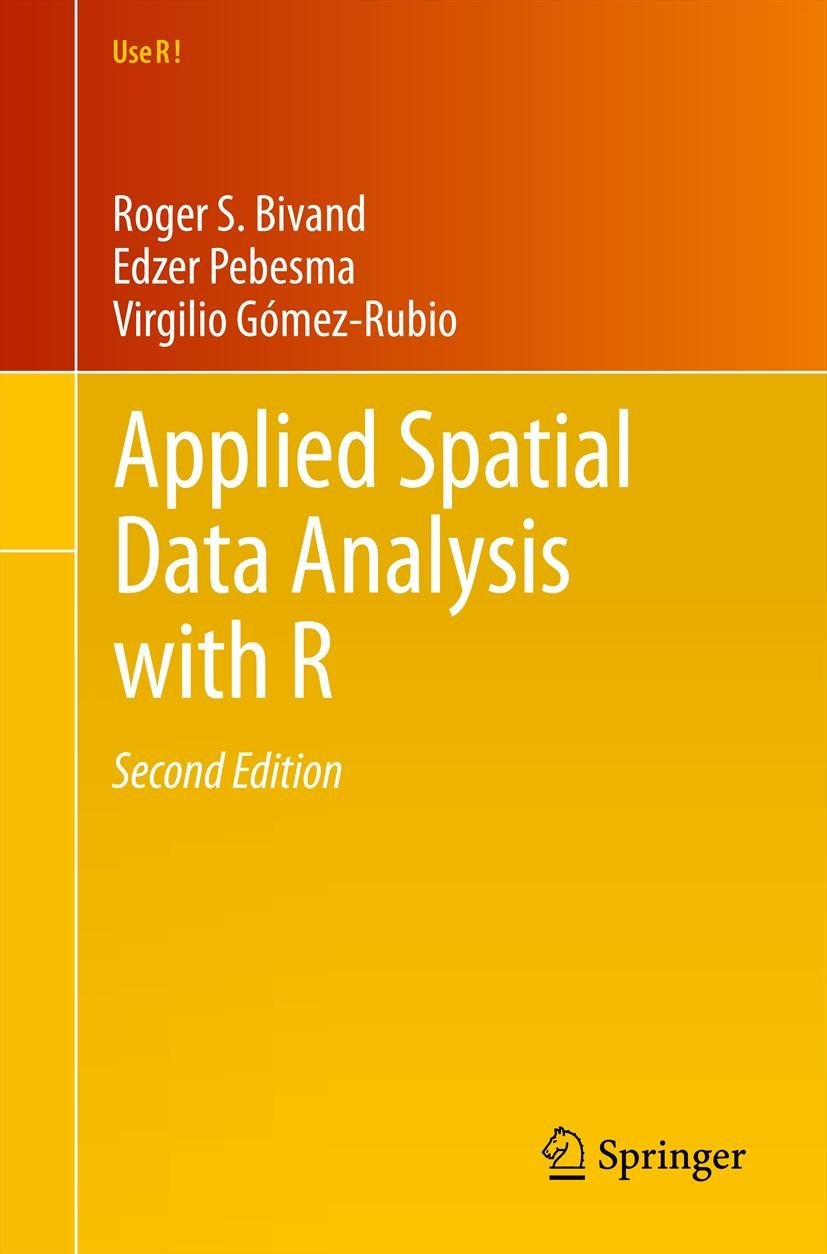
\includegraphics[width=0.3\linewidth]{../images/applied_spatial_data_analysis} \end{center}

\end{frame}

\begin{frame}{Additional Resources}

\textbf{Tutorials}

\begin{itemize}
\tightlist
\item
  \url{http://rpubs.com/RobinLovelace/11869}
\item
  \url{http://science.nature.nps.gov/im/datamgmt/statistics/r/advanced/spatial.cfm}
\item
  \url{http://spatial.ly/r/}
\item
  \url{http://gis.stackexchange.com/questions/45327/tutorials-to-handle-spatial-data-in-r}
\item
  \url{https://pakillo.github.io/R-GIS-tutorial/}
\end{itemize}

\textbf{R Spatial Cheatsheet}

\begin{itemize}
\tightlist
\item
  \url{http://www.maths.lancs.ac.uk/~rowlings/Teaching/UseR2012/cheatsheet.html}
\item
  \url{https://github.com/wegmann/RSdocs/releases/download/May2014_spatial/AniMove_refcard.pdf}
\end{itemize}

\end{frame}

\begin{frame}{Summary}

\begincols
\begincol{.69\textwidth}

\begin{enumerate}
\def\labelenumi{\arabic{enumi}.}
\tightlist
\item
  Help you get to the point where you can do basic analysis or
  visualization
\item
  Point out some of the commonly-used packages for spatial data
  manipulation and analysis
\item
  Be a resource you can come back to
\item
  Provide Guidance on useful resources to use after the course
\end{enumerate}

\endcol
\begincol{.3\textwidth}

\begin{center}
\includegraphics[width=1\linewidth]{../images/Goals} \end{center}

\endcol
\endcols

\begin{exampleblock}{}
Hopefully you have ticked a few of these boxes!
\end{exampleblock}

\end{frame}

\section{Thank You for Listening!}\label{thank-you-for-listening}

\end{document}